% AIXFil-Detect — IEEE Conference Paper
% Authors: Panhapiseth Lim, Halimat Popoola
% (Zulfiqar Khan commented out — add when ready)
% Dept. of Computer Science & Electrical Engineering
% The University of Texas Permian Basin

\documentclass[conference]{IEEEtran}

\usepackage{cite}
\usepackage{amsmath,amssymb,amsfonts}
\usepackage{graphicx}
\usepackage{textcomp}
\usepackage{xcolor}
\usepackage{booktabs}
\usepackage{microtype}
\usepackage{url}

% Space saving
\setlength{\textfloatsep}{6pt plus 2pt minus 2pt}
\setlength{\floatsep}{6pt plus 2pt minus 2pt}
\setlength{\intextsep}{6pt plus 2pt minus 2pt}

\begin{document}

% ─────────────────────────────────────────────────────────────────────────────
%  TITLE AND AUTHORS
% ─────────────────────────────────────────────────────────────────────────────

\title{AIXFil-Detect: Post-Hoc Forensic Attribution of Insider Data
       Exfiltration Through AI Chatbot Interfaces}

\author{%
  \IEEEauthorblockN{Panhapiseth Lim}
  \IEEEauthorblockA{%
    \textit{Dept.\ of Computer Science \& Electrical Engineering}\\
    \textit{The University of Texas Permian Basin}\\
    Odessa, TX 79762, USA\\
    lim\_p65274@utpb.edu}
  \and
  \IEEEauthorblockN{Halimat Popoola}
  \IEEEauthorblockA{%
    \textit{Dept.\ of Computer Science \& Electrical Engineering}\\
    \textit{The University of Texas Permian Basin}\\
    Odessa, TX 79762, USA\\
    popoola\_h51572@utpb.edu}
}

\maketitle

% ─────────────────────────────────────────────────────────────────────────────
%  ABSTRACT
% ─────────────────────────────────────────────────────────────────────────────

\begin{abstract}
Generative AI tools have introduced a data theft pathway that standard
security tools cannot see: an employee copies sensitive text from a
company file and pastes it into a browser-based chatbot. The file never
leaves the computer through a traditional channel, so no firewall or
data loss prevention system fires an alert. We present AIXFil-Detect,
an open-source forensic tool that reconstructs these events after the
fact by combining evidence from five Windows data sources: browser
history, the Windows clipboard database, file access timestamps, Windows
Prefetch execution logs, and network packet captures. Each group of
related events is scored with a Weighted Artifact Correlation Score
(WACS) that factors in evidence from each source, whether the clipboard
text matches the opened file, how much data was uploaded, and the time
of day. We tested the tool on 30 simulated scenarios and achieved
precision, recall, and F1 score of 1.00 at a WACS threshold of 75 using
a 30-second time window.
\end{abstract}

\begin{IEEEkeywords}
digital forensics, insider threat, AI chatbot security, Windows artifact
analysis, temporal correlation, data exfiltration
\end{IEEEkeywords}

% ─────────────────────────────────────────────────────────────────────────────
%  I. INTRODUCTION
% ─────────────────────────────────────────────────────────────────────────────

\section{Introduction}
\label{sec:intro}

Every day, employees at companies of all sizes copy confidential files
into browser-based AI chatbot tools. Payroll spreadsheets, legal
contracts, database exports, and customer records get pasted into a
chat window and sent to a remote server. The original file stays on the
employee's computer. Nothing goes out over email. Nothing is saved to a
USB drive. From the perspective of every standard security tool, the
user simply visited a website.

Data loss prevention (DLP) systems are built to monitor specific
channels: email, USB ports, cloud storage sync folders, and web proxies
that block known file-sharing sites. They look for outgoing content that
matches certain patterns, such as Social Security numbers or credit card
formats, or they watch for large file transfers to blocked
destinations~\cite{diro2025workplace}. The AI chatbot route bypasses all
of this. The destination is a normal HTTPS website that many companies
have already approved for employee use. The content being sent is just
text in a chat window, which looks identical to any other message. Once
an employee pastes company data into a chat interface, there is nothing
for a DLP tool to catch~\cite{gupta2023threatgpt}.

Network monitoring runs into the same problem. When a browser connects
to \texttt{chatgpt.com} or \texttt{claude.ai}, the connection uses TLS
encryption. The destination address is visible in the connection header,
but the content of the conversation is not. An employee asking a chatbot
to fix a grammar mistake and an employee submitting an entire customer
database look exactly the same to a network monitor~\cite{zhou2024tls}.

Insider threat research has been active for over two decades and has
produced many detection systems based on user behavior: login times,
file access patterns, volume of data read, and similar signals.
Al-Mhiqani et al.\ reviewed more than fifty of these systems and found
that almost all of them focus on a single stream of data at a
time~\cite{almhiqani2020review}. These systems are also real-time
monitors, which means they are good at raising alerts but poor at
reconstructing what happened after the fact. An investigator who needs
to prove that a specific employee copied a specific file into a specific
AI tool on a specific date cannot get that answer from a behavioral
alert. Breitinger et al.\ recently surveyed 150 papers on digital
forensics timeline reconstruction and noted that combining evidence from
multiple data sources at once, with an automated confidence score, is
still an open problem in the research community~\cite{breitinger2025sok}.

The closest prior work is by Cho et al., who studied what forensic
evidence the major AI chatbot applications leave behind on Windows,
iOS, and Android devices~\cite{cho2025conversational}. They catalog
where artifacts are stored for each platform and propose a checklist
for investigators. Their work is useful for knowing where to look, but
it does not answer whether any of those artifacts actually indicate
data theft. They do not score or combine evidence, and they do not
address the case where an employee is intentionally stealing data.

We built AIXFil-Detect to fill that gap. The tool reads forensic
evidence from five Windows data sources, groups events that happened
within 30 seconds of each other, and computes a WACS score that
summarizes how strong the evidence is. We tested it on 30 simulated
scenarios covering normal use, partial evidence, and clear exfiltration,
and it correctly classified all 30 with a precision, recall, and F1
score of 1.00. The source code and simulated dataset for AIXFil-Detect are openly available at \url{https://github.com/BryanLim0214/axifill}.

The rest of this paper is organized as follows. Section~\ref{sec:related}
covers related work. Section~\ref{sec:threat} describes the threat
model. Section~\ref{sec:design} explains the system design.
Section~\ref{sec:eval} presents the evaluation. Sections~\ref{sec:discussion}
through~\ref{sec:conclusion} discuss the results, limitations, and
conclusions.

% ─────────────────────────────────────────────────────────────────────────────
%  II. RELATED WORK
% ─────────────────────────────────────────────────────────────────────────────

\section{Related Work}
\label{sec:related}

\subsection{Insider Threat Detection and Timeline Forensics}

Most insider threat detection research builds models that watch a single
stream of data, such as login records, file access logs, or network
traffic. Al-Mhiqani et al.\ reviewed more than fifty of these systems,
covering classifiers ranging from support vector machines to neural
networks, and found that off-hours computer use is one of the most
reliable warning signs across nearly all of
them~\cite{almhiqani2020review}. Their review also notes a consistent
gap: these systems are designed for live monitoring, not for
reconstructing what a specific person did from saved evidence after an
incident has already occurred.

Breitinger et al.\ tackled this reconstruction problem in a large 2025
survey of 150 digital forensics timeline papers, published at the 25th
DFRWS conference~\cite{breitinger2025sok}. They found that 80.3\% of
forensic practitioners use timeline analysis in nearly every case, yet
there is no standardized way to combine timestamps from different data
sources, each of which uses different time formats and reference points.
They specifically called out automated confidence scoring based on
multiple corroborating sources as a direction the field has not yet
addressed. Our WACS score is a direct answer to that call.

\subsection{Windows Forensic Artifacts}

Each of the five data sources in AIXFil-Detect has been studied in
prior forensic research. Chand et al.\ tested forensic recovery from
Chrome, Edge, Firefox, Brave, and Opera on Windows and confirmed that
Chrome and Edge keep browsing history in a SQLite database file that
survives in forensic copies~\cite{chand2025browser}. They documented an
important technical detail: Chrome stores visit times as microseconds
counted from January 1, 1601, not from the standard Unix starting date
of January 1, 1970. To convert Chrome timestamps to standard time, you
divide by one million and subtract 11,644,473,600 seconds. This is
exactly what AIXFil-Detect's browser collector does.

Budhrani et al.\ analyzed Windows Prefetch files and confirmed that
each \texttt{.pf} file stores up to eight recent run times for the
associated program, a total run count, and a list of files the program
opened during its first ten seconds~\cite{budhrani2022prefetch}.
Prefetch files remain on disk even after the program is deleted, which
makes them useful for proving that a program ran in the past. Galhuber
and Luh tested how NTFS file timestamps behave across many different
file operations and showed that the \$STANDARD\_INFORMATION timestamp
can be changed by any user, while the \$FILE\_NAME timestamp can only
be changed at the operating system kernel level~\cite{galhuber2021ntfs}.
A mismatch between the two indicates that someone used a tool to fake
the timestamps, a technique known as timestomping. Javed et al.\
covered a broad range of Windows forensic topics and explained the
Windows Data Protection API (DPAPI) in detail: the encryption key is
tied to the user's login password, and without that password you need
either a RAM capture or a domain controller backup key to
decrypt~\cite{javed2022survey}. Each of these papers focuses on one
artifact type. None of them connects evidence across multiple sources
within a time window.

\subsection{AI Chatbot Forensics}

Cho et al.\ carried out the most thorough prior investigation of what
AI chatbots leave behind on a device~\cite{cho2025conversational}. They
examined ChatGPT, Gemini, Microsoft Copilot, and Claude across browser,
mobile, and desktop environments, documenting the browser history
records, cached responses, session cookies, and network traffic that
each platform generates. They also proposed a decision-tree guide for
investigators. Their contribution is essentially a catalog: here is
what exists, and here is where to find it. What they do not address is
the question of what the evidence means. They provide no scoring system,
no way to combine artifacts from different sources, and no analysis of
the scenario where an employee is deliberately trying to steal data.
AIXFil-Detect picks up where their work ends.

Kankanamge et al.\ studied the ChatGPT Windows desktop application
specifically and found that clipboard data from chatbot sessions can
be recovered from Windows memory, and that the size of HTTPS uploads
to the OpenAI server grows with the amount of text the user
submitted~\cite{kankanamge2025chatgpt}. Both of these findings are
directly relevant to AIXFil-Detect: the clipboard collector reads the
Windows clipboard history database, and the network collector uses
upload size as one of its scoring factors.

\subsection{Network Traffic and Content Matching}

Even though TLS 1.3 encrypts the content of web connections, the
Server Name Indication (SNI) field in the connection setup is still
sent in plain text for most websites today. This is because the
technology that would hide SNI, called Encrypted ClientHello (ECH),
has not yet been adopted widely on the server side~\cite{zhou2024tls}.
Zhou et al.\ confirmed in their 2024 survey that SNI is still usable
for identifying AI chatbot connections, and that the total size of an
encrypted upload can be estimated from packet sizes even without
decrypting the content.

For content matching between clipboard text and file contents, we use
MinHash, a technique introduced by Broder in 1997~\cite{broder1997minhash}.
The core idea is that two documents can be compared without reading
every word. Instead, each document is broken into overlapping
three-character pieces called shingles, and a hash function picks a
minimum value from those pieces. If two documents have similar content,
their minimum hash values will match with a probability equal to their
Jaccard similarity score. Using 128 hash functions gives an error of
about $\pm$9\%, which is accurate enough for our purposes and runs
very quickly even on large files.

% ─────────────────────────────────────────────────────────────────────────────
%  III. THREAT MODEL
% ─────────────────────────────────────────────────────────────────────────────

\section{Threat Model}
\label{sec:threat}

The insider in this model is an employee who has normal, legitimate
access to sensitive files at their company. They may be using an
AI chatbot that the company has approved, or they may be using a
personal account on a public service. Either way, their goal is to get
sensitive information out of the organization by pasting it into the
AI chat interface and accessing it later through that platform or
some other means.

The sequence of steps is short. The employee opens a sensitive file,
such as a payroll spreadsheet or a contract, selects the content they
want, and copies it. They then open a browser, go to an AI chatbot
site, paste the text into the prompt box, and click send. The whole
process takes less than a minute. After that, the data lives on
a server the company does not control.

\begin{figure}[!htbp]
  \centerline{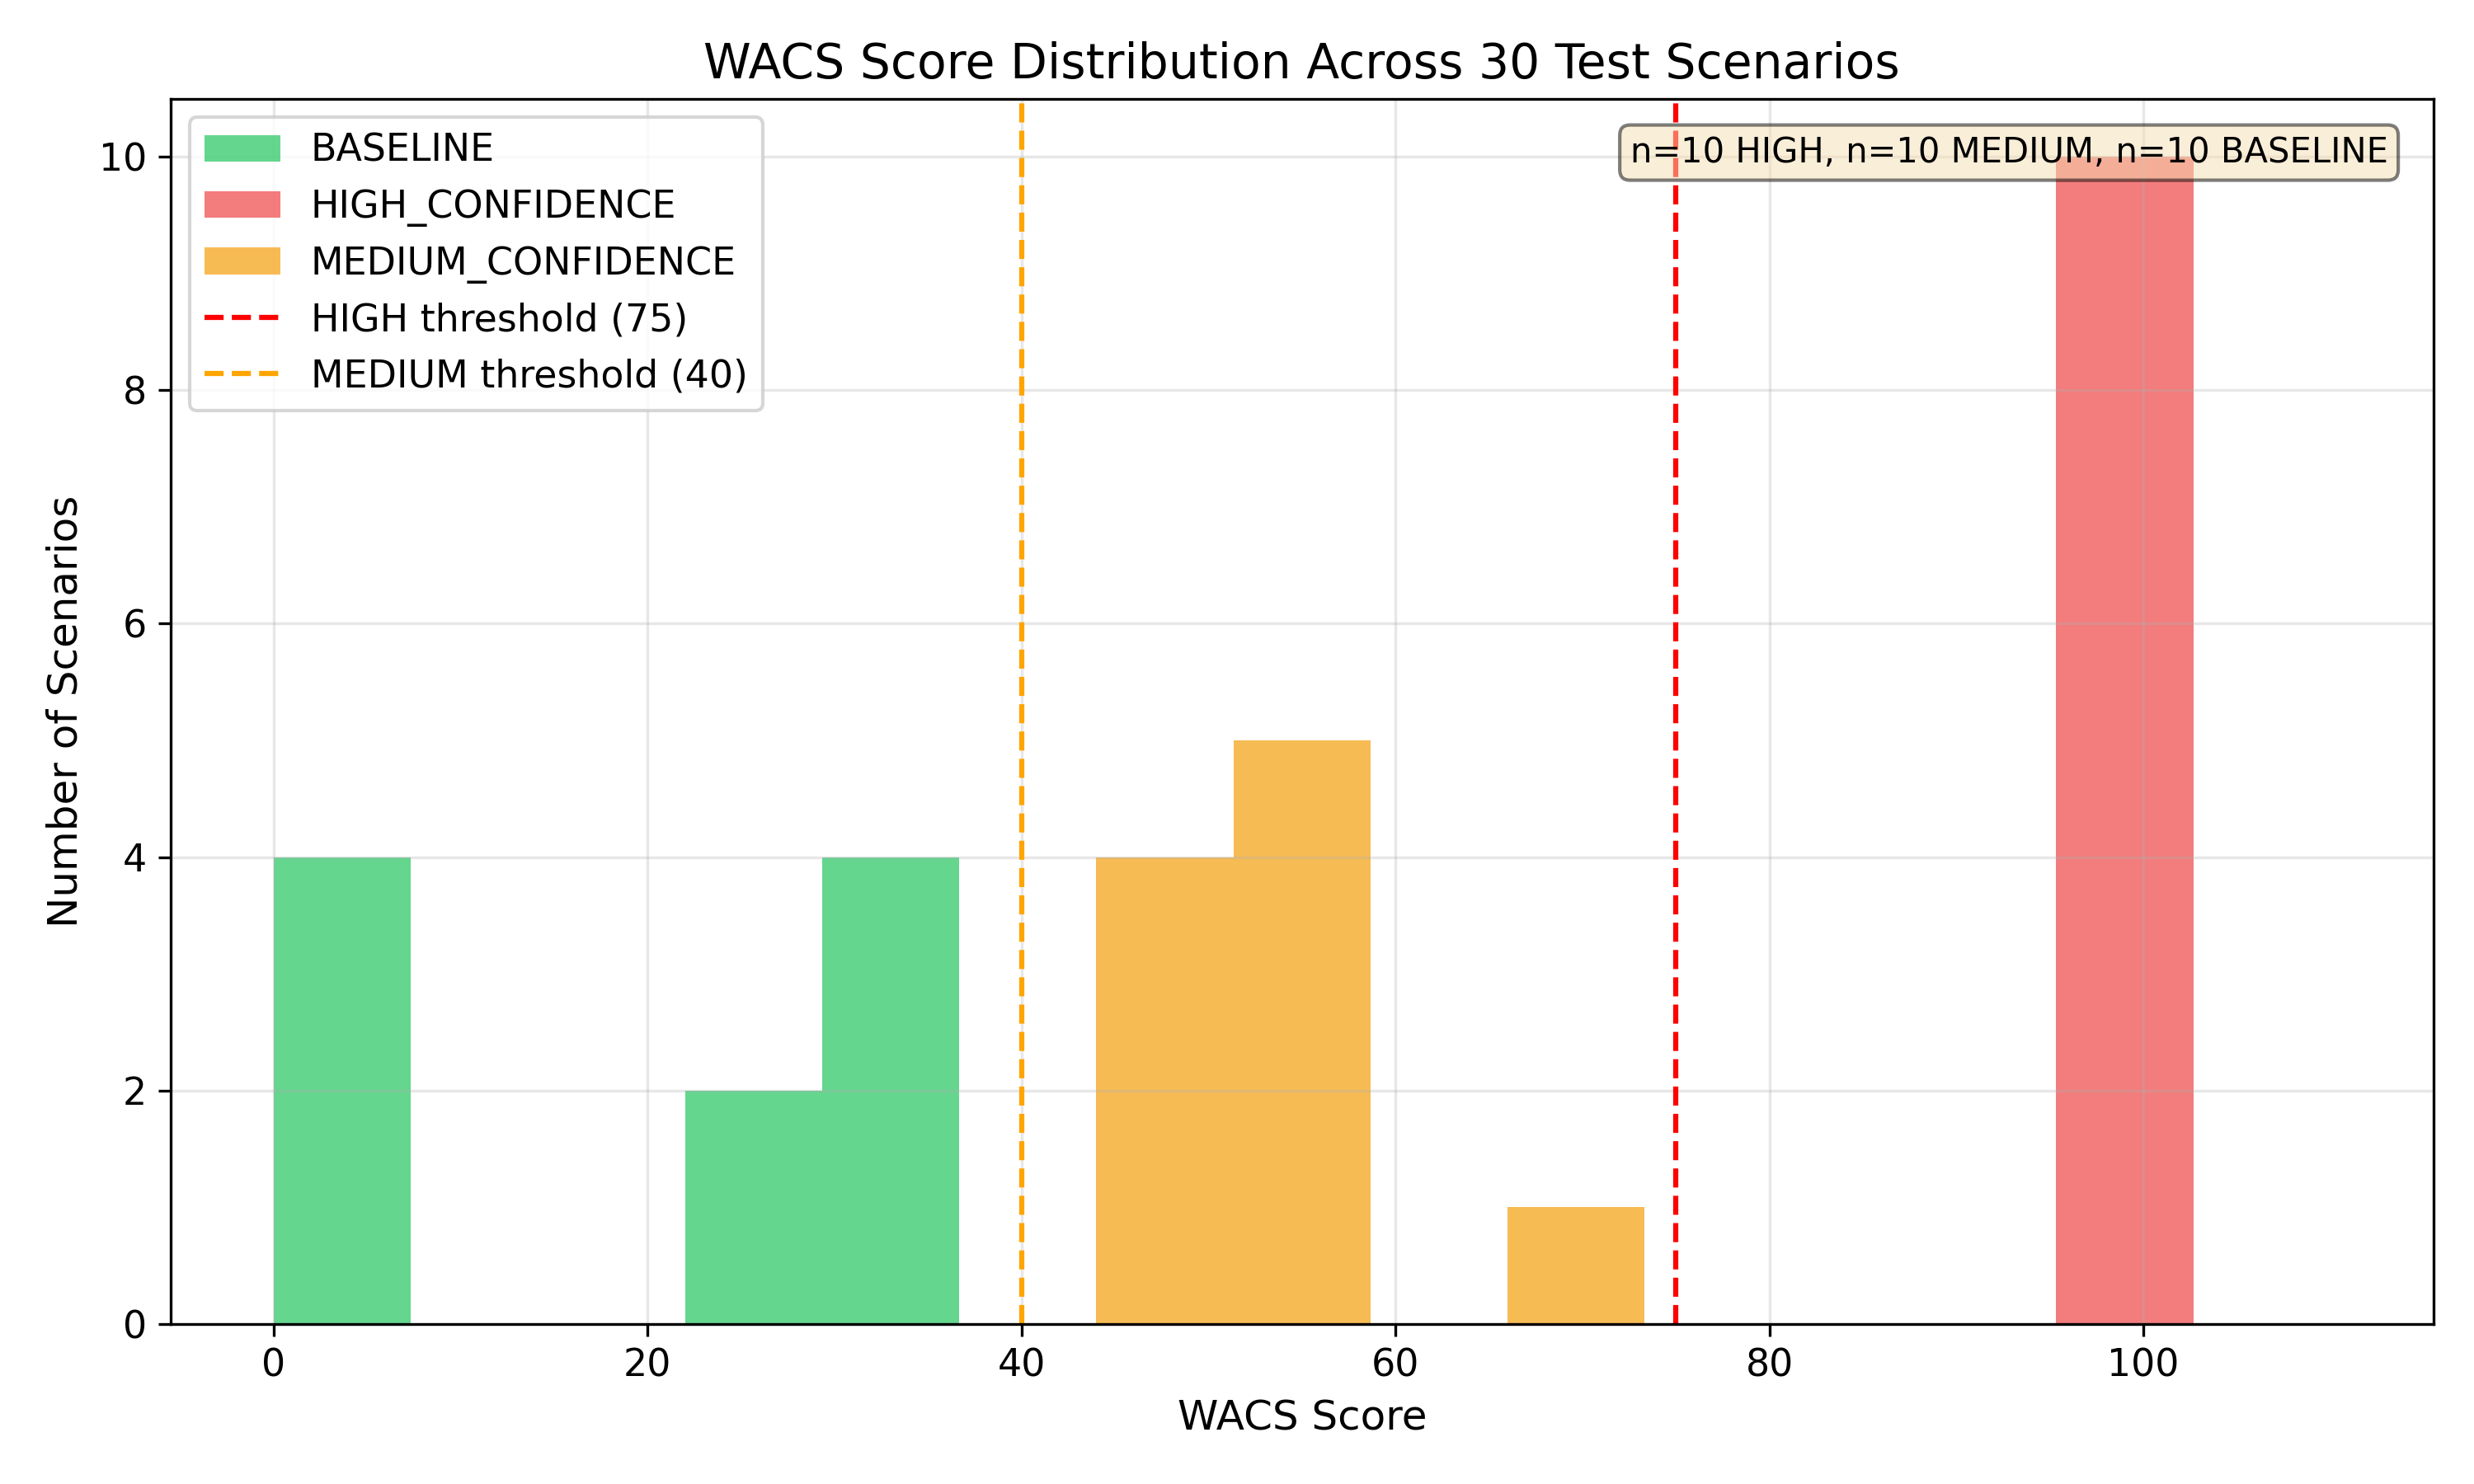
\includegraphics[width=0.9\columnwidth]{figures/fig1_wacs_distribution}}
  \caption{WACS score distribution for all 30 scenarios at the 30-second
  window. HIGH scenarios (red) all score 100. MEDIUM (orange) and BASELINE
  (green) are clearly separated.}
  \label{fig:wacs_dist}
\end{figure}
Standard security tools miss this because they each look at only one
thing at a time. DLP systems look at outbound file transfers and email
attachments, not at text typed into a chat window~\cite{diro2025workplace}.
Network monitors see a connection to an approved website, but since
the content is encrypted, they cannot tell whether the employee sent
a one-line question or a 5,000-word document~\cite{gupta2023threatgpt}.
No single piece of evidence, looked at on its own, is enough to raise
an alarm.

AIXFil-Detect works by looking at everything together. A visit to an
AI website is not suspicious by itself. A large chunk of text in the
clipboard is not suspicious by itself. A recently opened payroll file
is not suspicious by itself. But all three happening within 30 seconds
of each other tells a clear story that an investigator can act on.

% ─────────────────────────────────────────────────────────────────────────────
%  IV. SYSTEM DESIGN
% ─────────────────────────────────────────────────────────────────────────────

\section{System Design}
\label{sec:design}

\subsection{Architecture Overview}

AIXFil-Detect works in four stages: collection, grouping, scoring, and
reporting. First, five separate collectors each read one data source and
produce a list of time-stamped events. Second, a grouping step takes
all these events, finds browser visits to AI websites, and pulls in
any related events from the other collectors that happened within the
time window. Third, a scoring function assigns a WACS score to each
group of events. Fourth, everything is written into an HTML report that
an investigator can open in any browser.

\begin{figure}[!htbp]
  \centerline{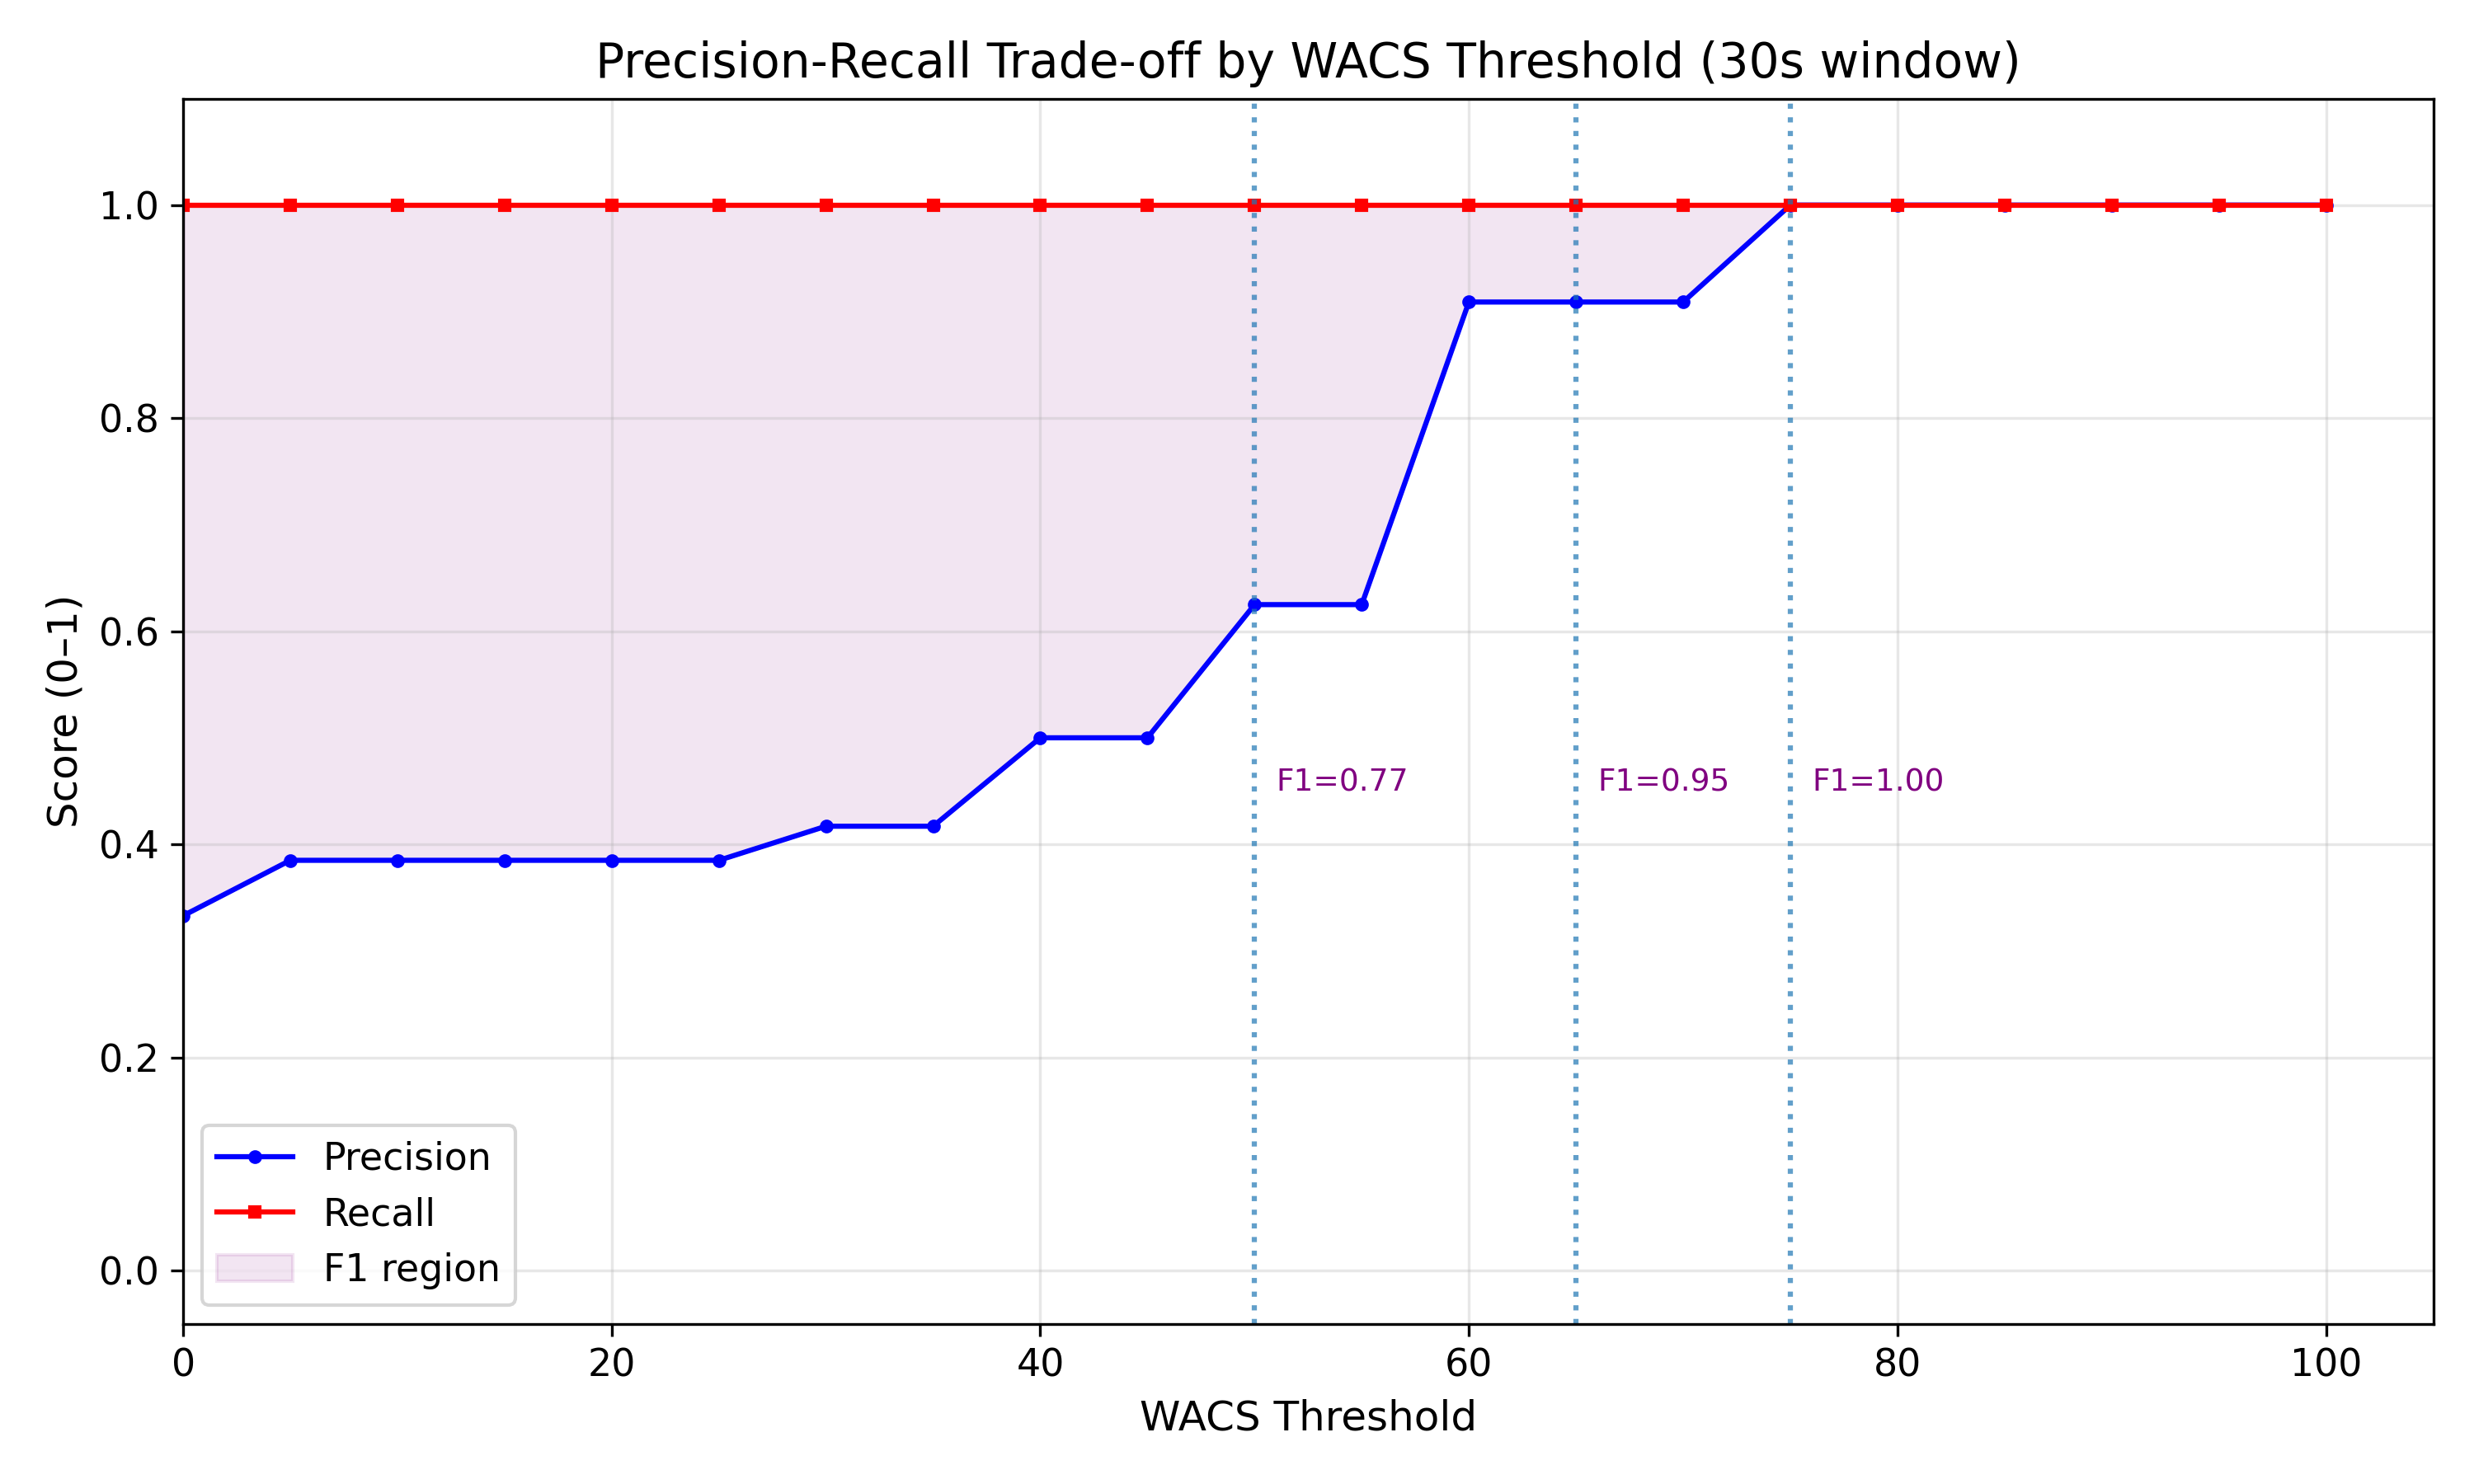
\includegraphics[width=0.9\columnwidth]{figures/fig2_precision_recall_curve}}
  \caption{Precision and recall vs.\ WACS threshold at the 30-second
  window. Recall stays at 1.000 across all thresholds.}
  \label{fig:pr_curve}
\end{figure}
\subsection{Layer 1: Browser History Collector}

Chrome and Edge store browsing history in a SQLite database file called
\texttt{History}, located in the user's application data
folder~\cite{chand2025browser}. The collector reads each visit record
and converts the timestamp from Chrome's internal format to standard
Unix time using the formula:
$t_{\text{unix}} = t_{\text{chrome}}/10^{6} - 11{,}644{,}473{,}600$.
Chrome stores time as microseconds since January 1, 1601. Dividing by
one million converts to seconds, and subtracting the constant shifts the
starting point to the standard Unix epoch of January 1, 1970.

The collector then checks whether the website matches any of the 14 AI
domains on its list, including \texttt{chatgpt.com}, \texttt{claude.ai},
\texttt{gemini.google.com}, and \texttt{copilot.microsoft.com}. When a
visit is the user's first time going to that AI site, the scorer awards
a bonus because an employee visiting an AI platform for the first time
while working with sensitive files is more noteworthy than someone who
goes there every day.

\subsection{Layer 2: Clipboard Collector}

Windows saves clipboard history in a SQLite database that the
ClipboardService process maintains in the user's local application data
folder. The collector reads each saved entry. Before trying to read the
content as text, it checks the first eight bytes for the signature
\texttt{01\,00\,00\,00\,D0\,8C\,9D\,DF}. If those bytes are present,
the entry is encrypted with DPAPI and cannot be read without the user's
Windows password~\cite{javed2022survey}.

If the clipboard entry is readable text longer than 100 bytes, it gets
30 points (meaningful portion). If it is readable but shorter than 100
bytes, or if it is DPAPI-encrypted, it gets 10 points
(corroboration)~\cite{kankanamge2025chatgpt}.

\begin{figure}[!htbp]
  \centerline{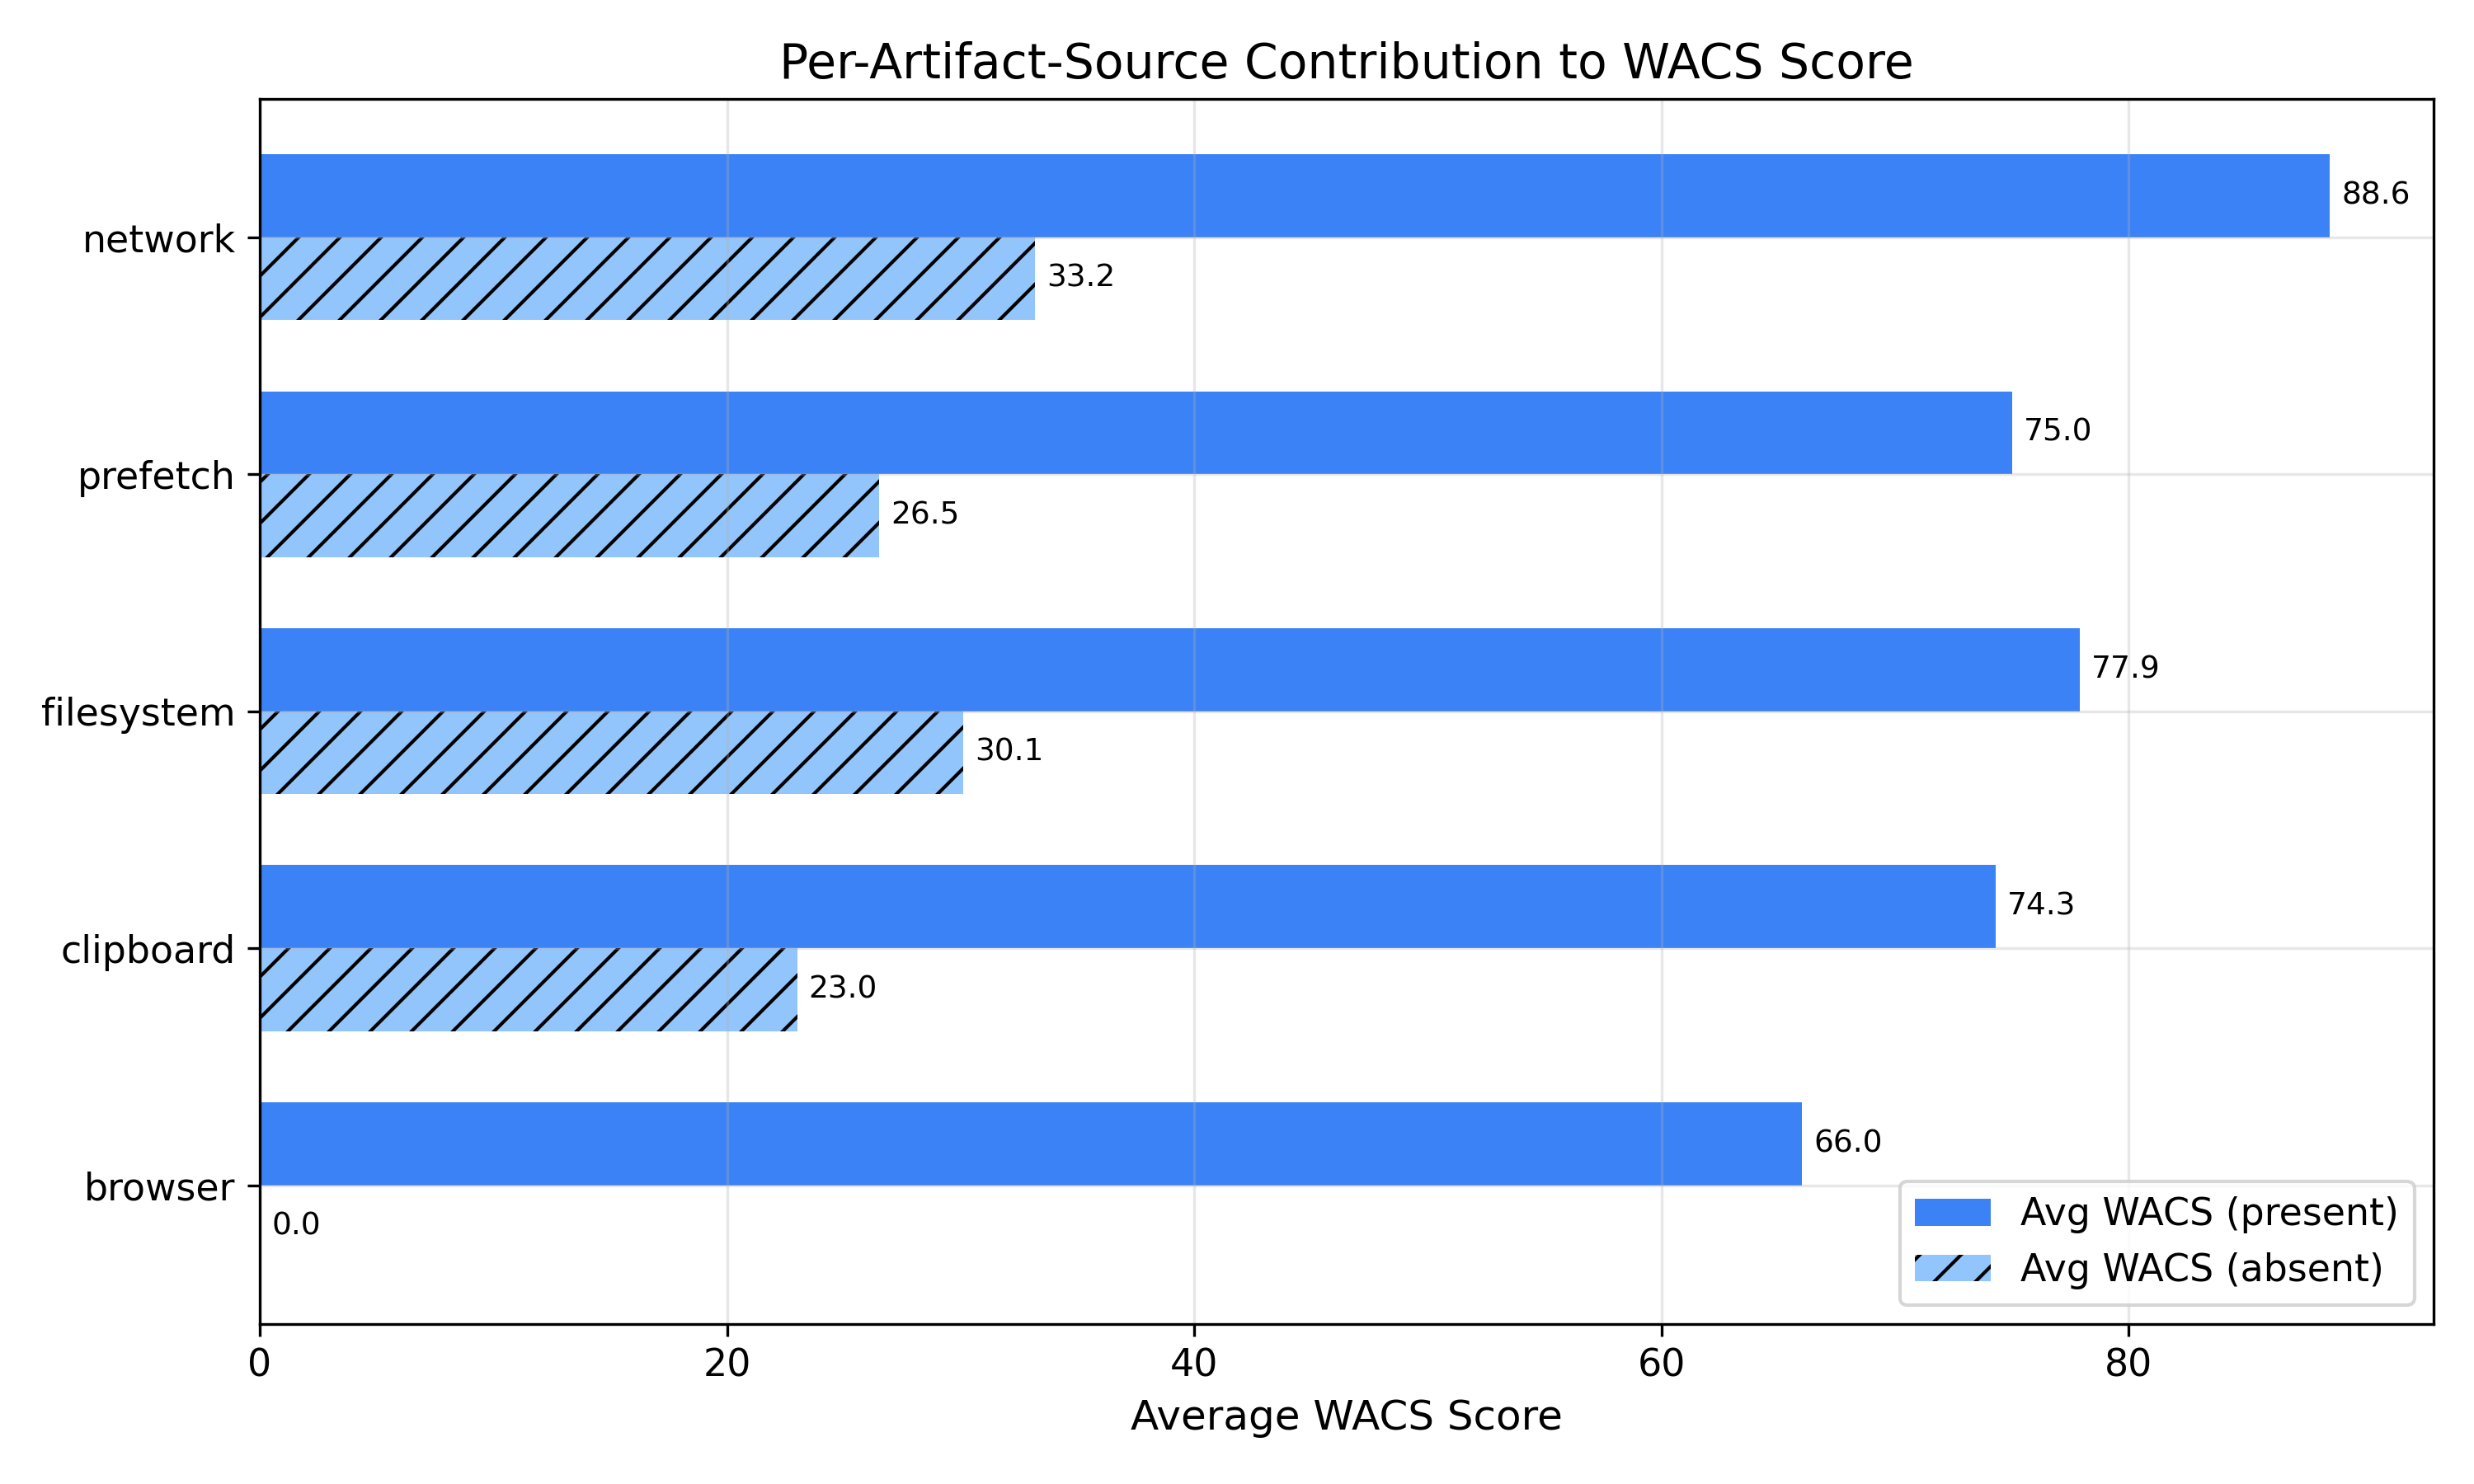
\includegraphics[width=0.9\columnwidth]{figures/fig3_source_contribution}}
  \caption{Average WACS when each data source is present versus absent.
  The clipboard produces the largest score difference (51.3 points).}
  \label{fig:source_contrib}
\end{figure}


\subsection{Layer 3: Filesystem Collector}

The filesystem collector looks at when files were last accessed in a
target directory. It flags files with sensitive extensions:
\texttt{.xlsx}, \texttt{.csv}, \texttt{.pdf}, \texttt{.docx},
\texttt{.sql}, \texttt{.bak}, \texttt{.pfx}, \texttt{.pem},
\texttt{.key}, and \texttt{.cer}. Certificate and key files get an
additional high-value flag because they are damaging to lose.

Windows turns off last-access updates by default to improve
performance~\cite{galhuber2021ntfs}. The collector checks this setting
and reports Layer 3 as unavailable if it is disabled.

\subsection{Layer 4: Prefetch Collector}

Every time a program runs on Windows, the operating system creates or
updates a Prefetch file in \texttt{C:\textbackslash Windows\textbackslash
Prefetch}. Each file stores up to eight recent run times, a run count,
and a list of files opened during the first ten
seconds~\cite{budhrani2022prefetch}.

The Prefetch timestamp is recorded about ten seconds after the program
actually launched. The collector subtracts ten seconds to get an
accurate launch time. Points are added only when a document application
and a browser both ran around the same time, preventing false positives
from routine browsing.

\subsection{Layer 5: Network PCAP Collector}

The network collector reads PCAP files and looks for TLS connections to
AI websites. Handshake SNIs are still sent in plain text even in TLS
1.3~\cite{zhou2024tls}. The collector uses Scapy to parse the SNI or
searches raw packet bytes for known AI domains.

For each connection, the collector adds up total bytes sent. A base score
of 15 points is awarded for any AI upload. An extra 10 points are added
if the upload exceeds 100 KB (document-sized).

\begin{figure}[!htbp]
  \centerline{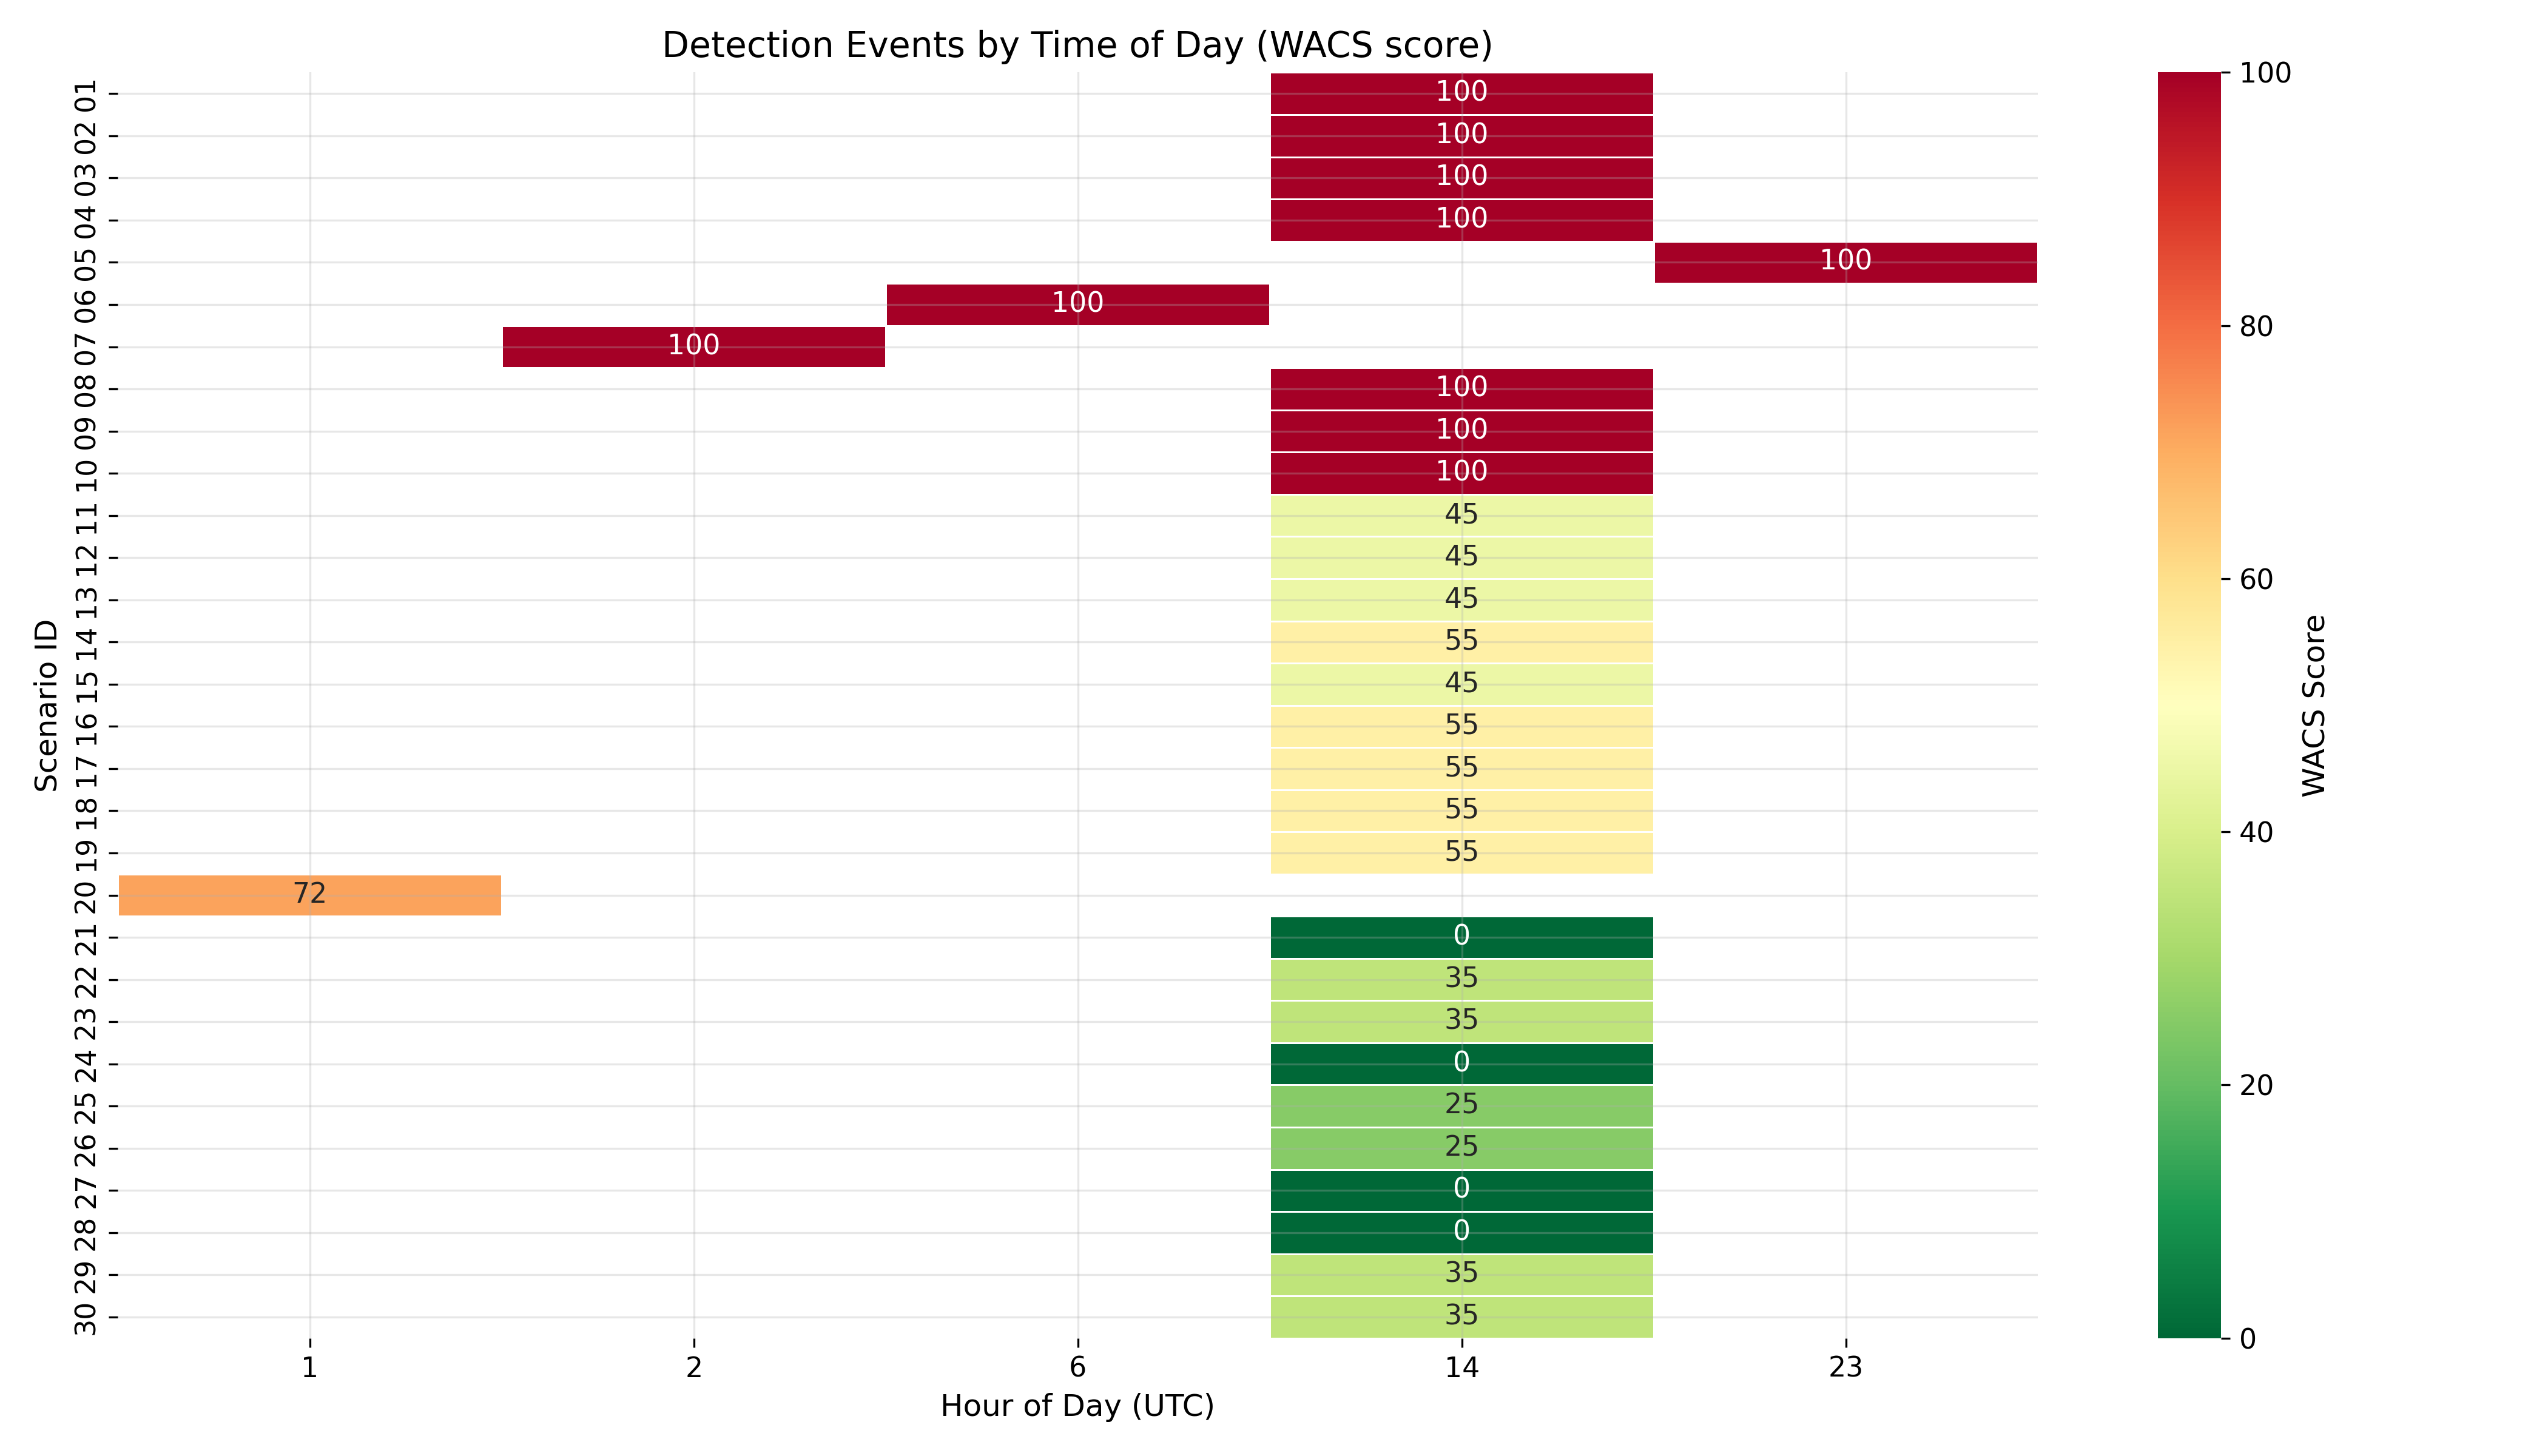
\includegraphics[width=0.9\columnwidth]{figures/fig4_timeline_heatmap}}
  \caption{Hour-of-day distribution for all 30 scenarios, colored by WACS
  score. Off-hours HIGH scenarios reach WACS = 100.}
  \label{fig:heatmap}
\end{figure}
\subsection{Temporal Correlator}

The correlator merges all events into one list sorted by time. It
gathers all events within $W$ seconds (default 30) of a browser visit
to an AI domain. Groups with events from two or more sources are kept
for scoring. All timestamps are normalized to standard Unix seconds
before grouping~\cite{breitinger2025sok}.



\subsection{WACS Scorer}

Each cluster receives a WACS score:
$\text{WACS} = \min(100, (\sum w_{s} + b_{\text{clip}} + b_{\text{net}} + b_{\text{visit}}) \times m_{\text{hrs}})$.
$\mathcal{S}$ is the set of contributing sources, $w_s$ are base points,
and $b$ are bonus terms for matches, large uploads, and new domains.
$m_{\text{hrs}}$ raises the score by 30\% for off-hours activity. Table~\ref{tab:weights}
lists all weights.

\begin{table}[t]
  \caption{WACS Component Weights and Scoring Conditions}
  \label{tab:weights}
  \begin{center}
  \begin{tabular}{lcc}
    \toprule
    \textbf{Component} & \textbf{Points} & \textbf{Condition} \\
    \midrule
    Browser visit          & 25          & AI domain confirmed \\
    Clipboard entry        & 30          & Readable text $>$100 bytes \\
    Clipboard (partial)    & 10          & Encrypted or short content \\
    Filesystem access      & 20          & Sensitive file extension \\
    Prefetch record        & 10          & Doc app + browser both ran \\
    Network upload         & 15          & AI-domain upload confirmed \\
    Content match bonus    & up to $+$20 & Jaccard $\geq$0.5~\cite{broder1997minhash} \\
    Large-upload bonus     & $+$10       & Upload exceeds 100 KB \\
    New-domain bonus       & $+$10       & First visit to that AI site \\
    Off-hours multiplier   & $\times$1.3 & Before 08:00 or after 18:00 \\
    \midrule
    \multicolumn{3}{l}{\footnotesize
      HIGH $\geq 75$;\quad MEDIUM 40--74;\quad BASELINE $<$ 40.} \\
    \bottomrule
  \end{tabular}
  \end{center}
\end{table}

We use MinHash~\cite{broder1997minhash} to compare clipboard text
against file content. A similarity score $\geq 0.5$ triggers up to 20
bonus points. Clusters score HIGH (75+), MEDIUM (40--74), or
BASELINE ($<$40).

\begin{figure}[!htbp]
  \centerline{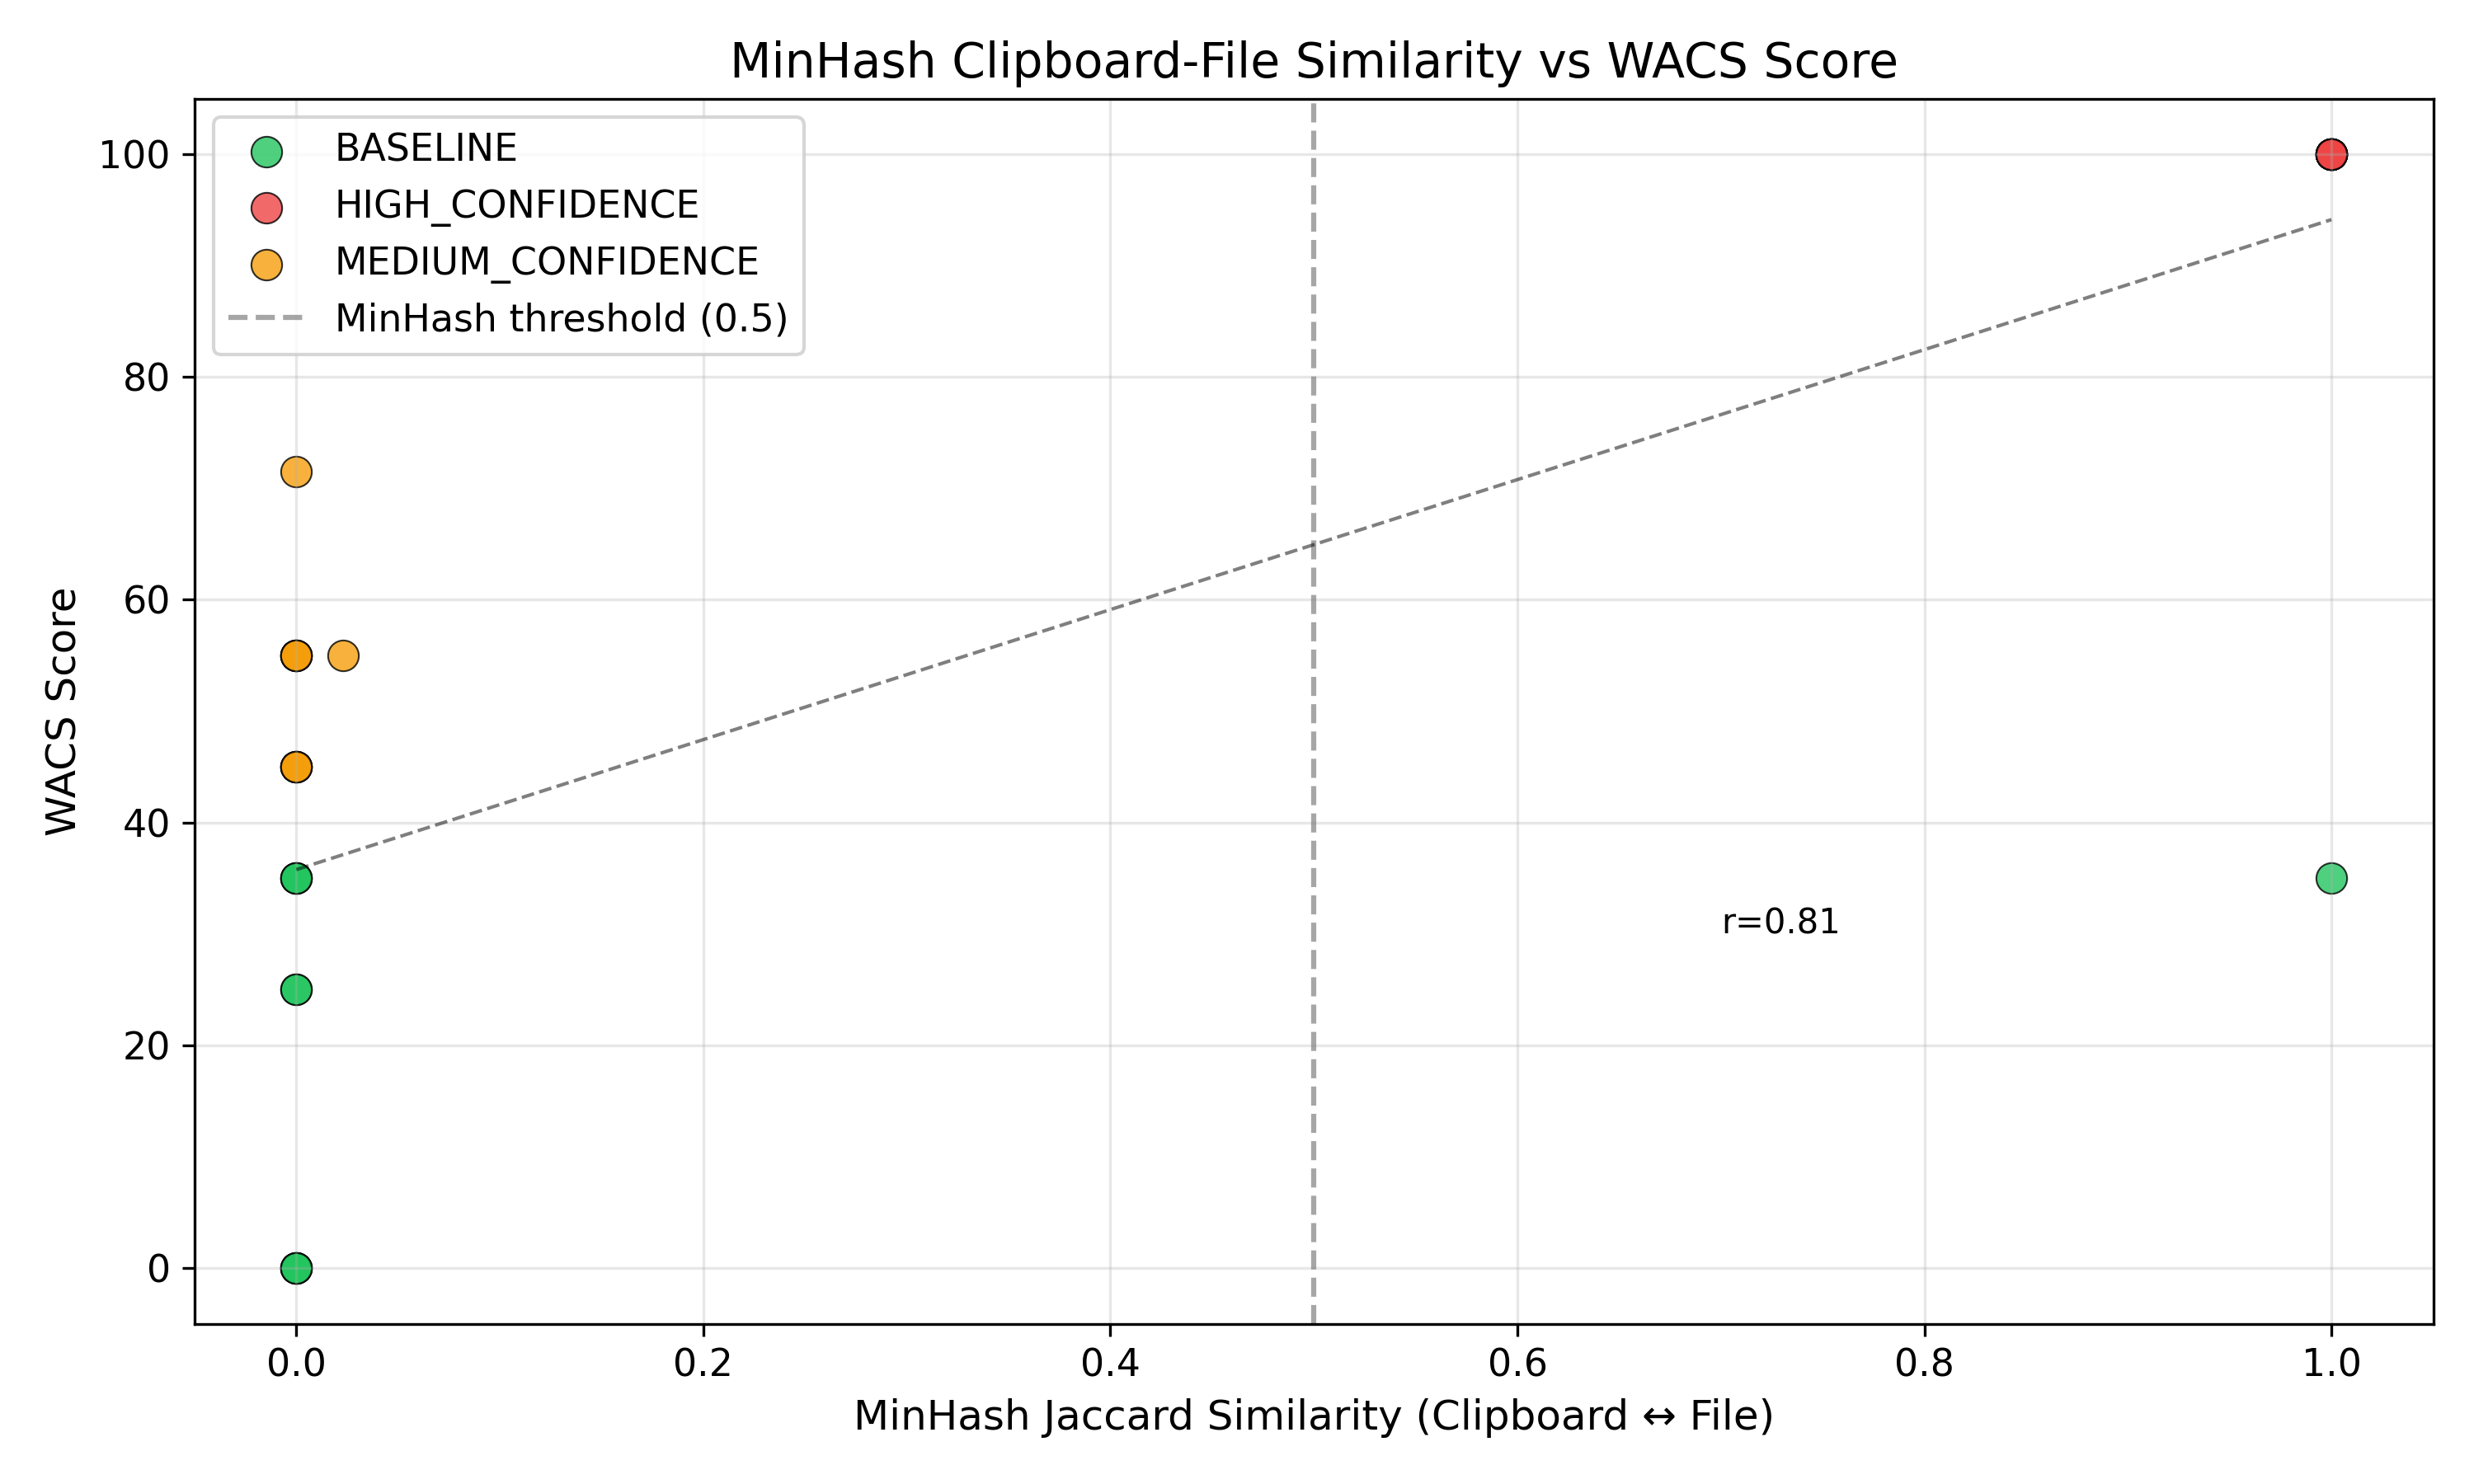
\includegraphics[width=0.9\columnwidth]{figures/fig5_minhash_scatter}}
  \caption{MinHash Clipboard-File similarity vs.\ WACS score. HIGH
  scenarios (orange) cluster at similarity = 1.0 and WACS = 100.}
  \label{fig:minhash}
\end{figure}


\subsection{Anti-Forensics Detection}

When MFT data is available, the tool compares
\$STANDARD\_INFORMATION and \$FILE\_NAME NTFS
timestamps~\cite{galhuber2021ntfs}. Gaps in browser history, cleared
clipboard entries, or Prefetch anomalies also trigger warning flags.
These do not change the WACS score but appear in the report.

\begin{figure}[!htbp]
  \centerline{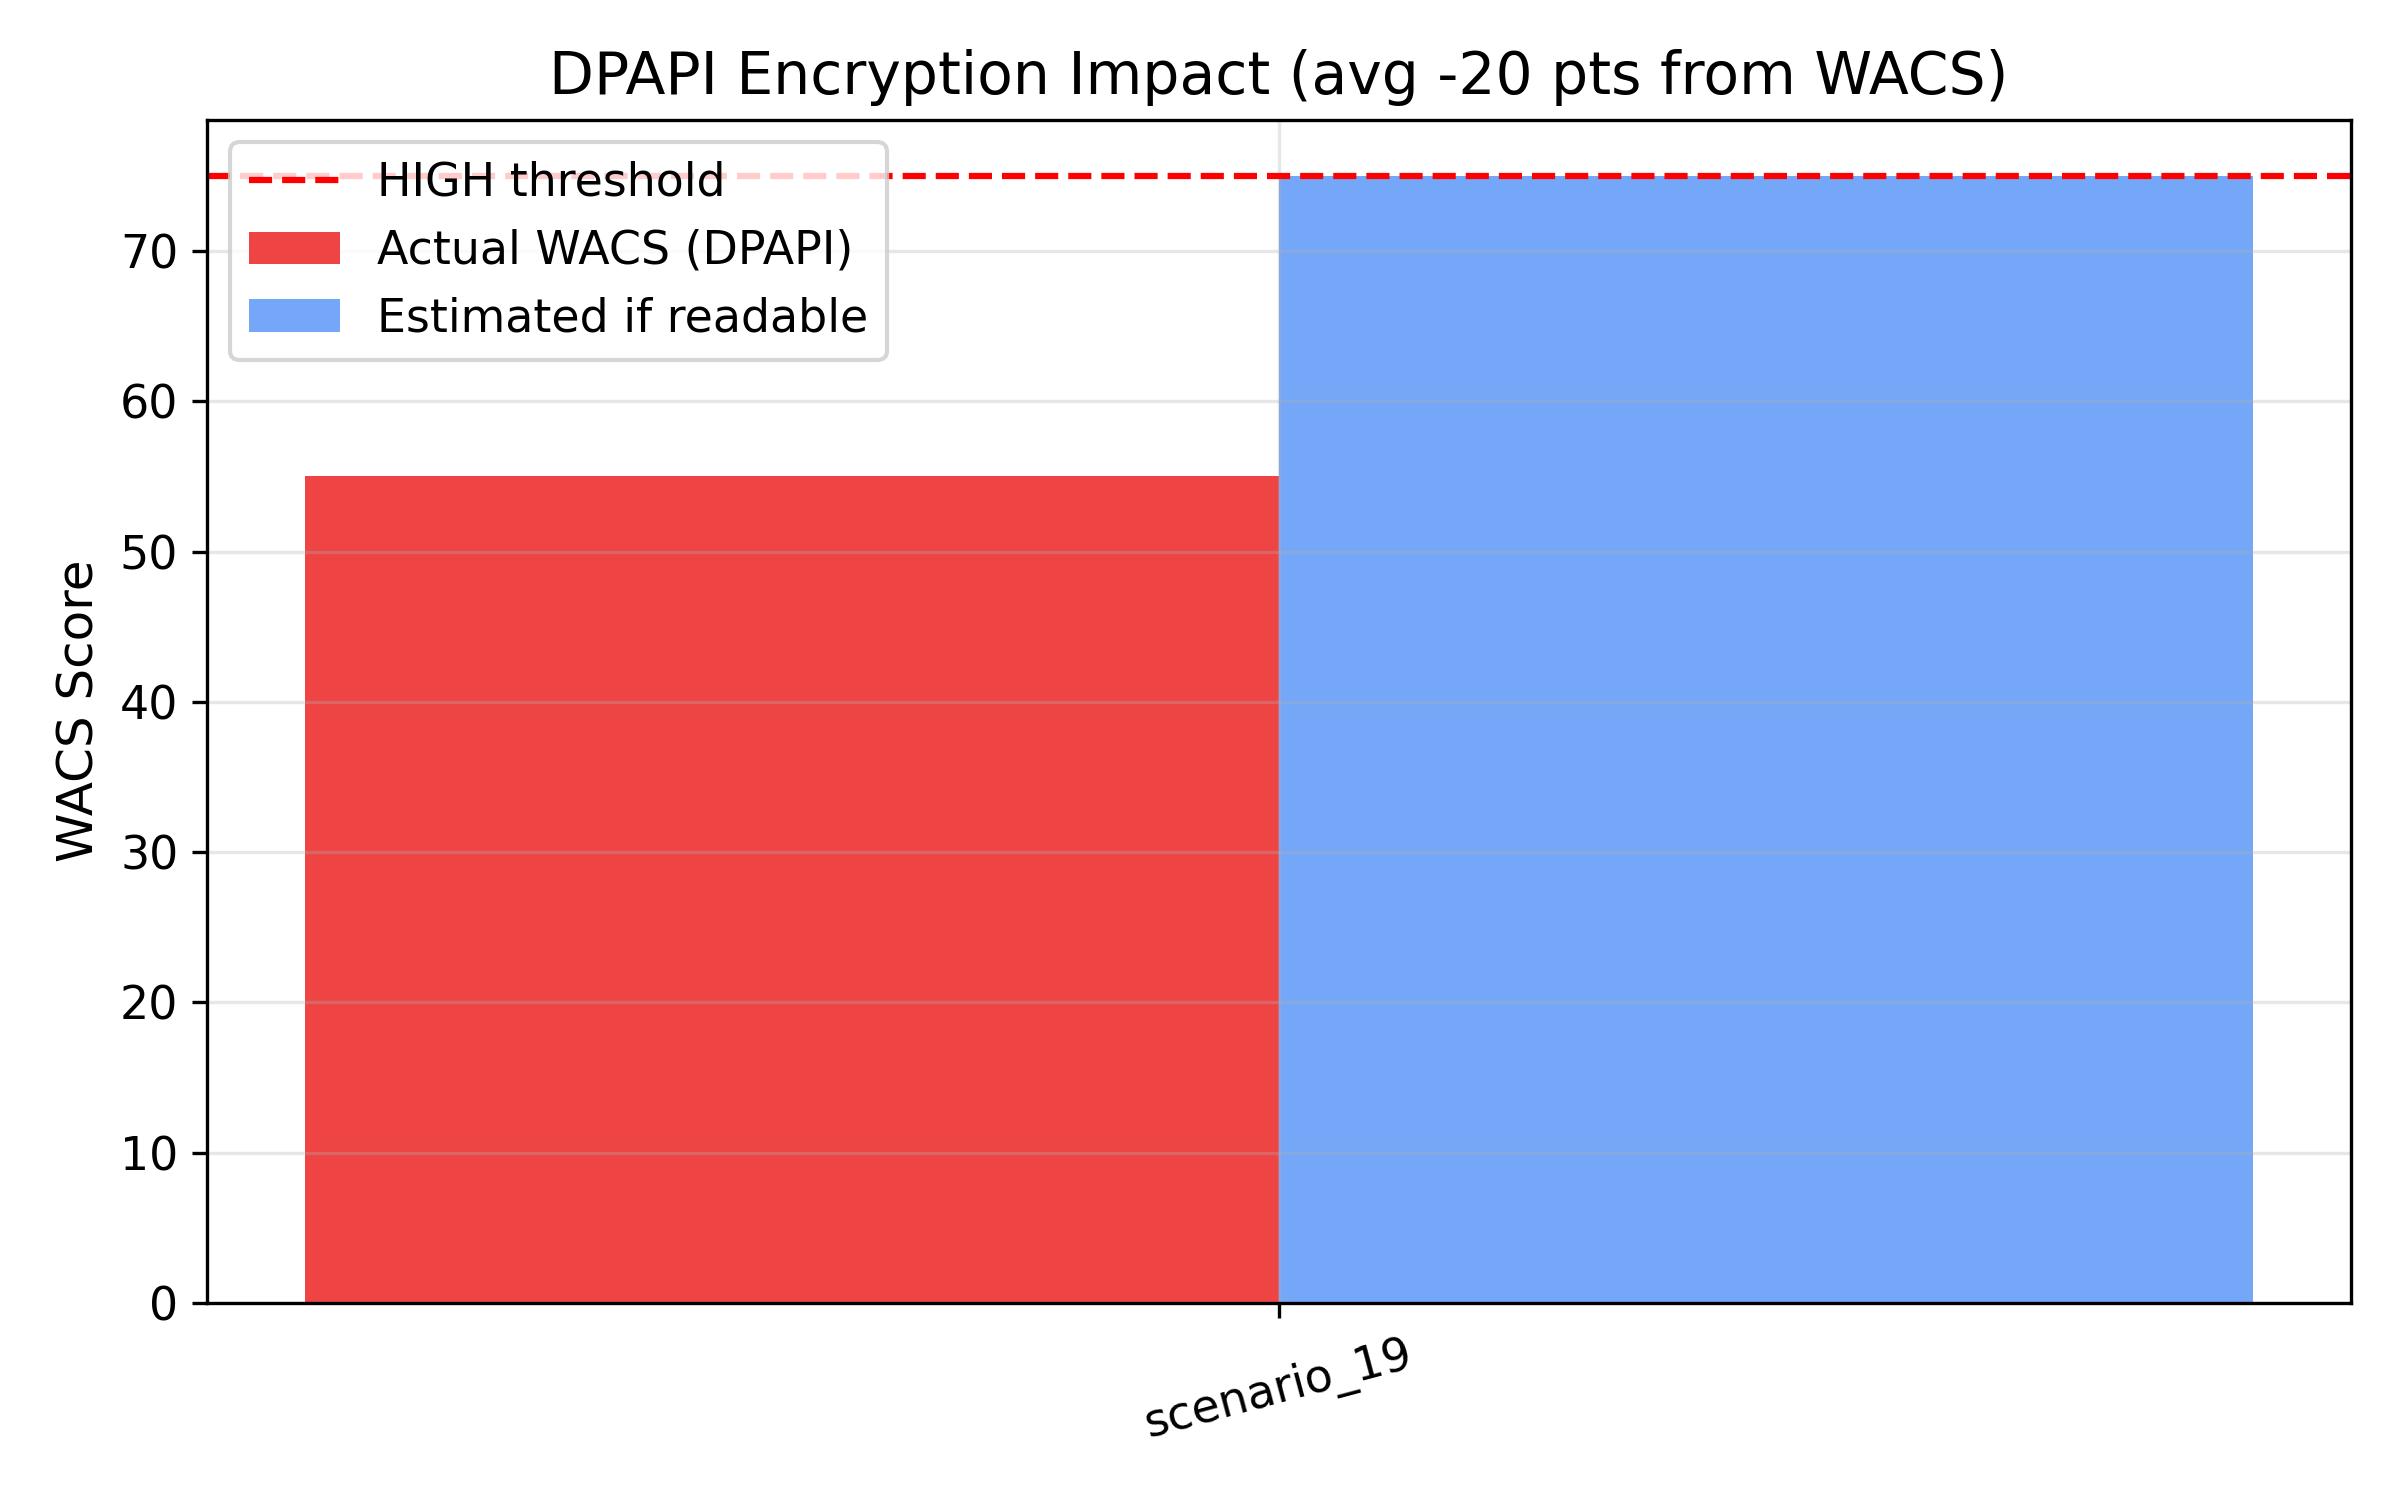
\includegraphics[width=0.9\columnwidth]{figures/fig6_dpapi_impact}}
  \caption{Actual WACS (gray) vs.\ estimated WACS if clipboard were
  readable (orange) for DPAPI-affected scenarios.}
  \label{fig:dpapi}
\end{figure}


% ─────────────────────────────────────────────────────────────────────────────
%  V. EXPERIMENTAL EVALUATION
% ─────────────────────────────────────────────────────────────────────────────

\section{Experimental Evaluation}
\label{sec:eval}

\subsection{Simulation Design}

We built a simulator that generates realistic forensic artifacts for 30
defined test scenarios (10 HIGH, 10 MEDIUM, 10 BASELINE). Scenarios
cover six file types (.xlsx, .pdf, .py, .sql, .pfx, .csv) and six AI
platforms. AIXFil-Detect reads the generated SQLite, JSON, and PCAP
files through the same code path used for real forensic images.



\subsection{Results}



\begin{table*}[t]
  \begin{minipage}{0.48\textwidth}
    \caption{Representative Scenario Results (30 s Window, Threshold = 75)}
    \label{tab:results}
    \begin{center}
    \footnotesize
    \begin{tabular}{lccccc}
      \toprule
      \textbf{Scenario} & \textbf{Exp.} & \textbf{Act.} &
      \textbf{WACS} & \textbf{Res.} & \textbf{Sim.} \\
      \midrule
      01: payroll, claude.ai    & H & H & 100 & TP & 1.00 \\
      07: cert, off-hours 02:00 & H & H & 100 & TP & 1.00 \\
      08: 150\,KB upload        & H & H & 100 & TP & 1.00 \\
      10: customer list         & H & H & 100 & TP & 1.00 \\
      11: clipboard missed win. & M & M &  45 & TN & 0.00 \\
      16: short clipboard       & M & M &  55 & TN & 0.00 \\
      19: DPAPI encrypted       & M & M &  55 & TN & 0.00 \\
      20: near threshold        & M & M &  72 & TN & 0.00 \\
      21: normal browsing       & B & B &   0 & TN & 0.00 \\
      30: non-sensitive file    & B & B &  35 & TN & 1.00 \\
      \bottomrule
      \multicolumn{6}{l}{H\,=\,HIGH; M\,=\,MED; B\,=\,BASE; Sim.\,=\,MinHash.}
    \end{tabular}
    \end{center}
  \end{minipage}\hfill
  \begin{minipage}{0.48\textwidth}
    \caption{Classification Performance by Threshold and Window}
    \label{tab:pr}
    \begin{center}
    \begin{tabular}{ccccc}
      \toprule
      \textbf{Threshold} & \textbf{Window} &
      \textbf{Precision} & \textbf{Recall} & \textbf{F1} \\
      \midrule
      50 & 30 s & 0.625 & 1.000 & 0.769 \\
      50 & 60 s & 0.500 & 1.000 & 0.667 \\
      65 & 30 s & 0.909 & 1.000 & 0.952 \\
      65 & 60 s & 0.588 & 1.000 & 0.741 \\
      \textbf{75} & \textbf{30 s} & \textbf{1.000} & \textbf{1.000} & \textbf{1.000} \\
      75 & 60 s & 0.833 & 1.000 & 0.909 \\
      \bottomrule
    \end{tabular}
    \end{center}
  \end{minipage}
\end{table*}

At threshold 75 and 30-second window, the tool achieved precision,
recall, and F1 of 1.00 (Table~\ref{tab:pr}). HIGH scenarios separated
perfectly from MEDIUM and BASELINE tiers.

\begin{figure}[!htbp]
  \centerline{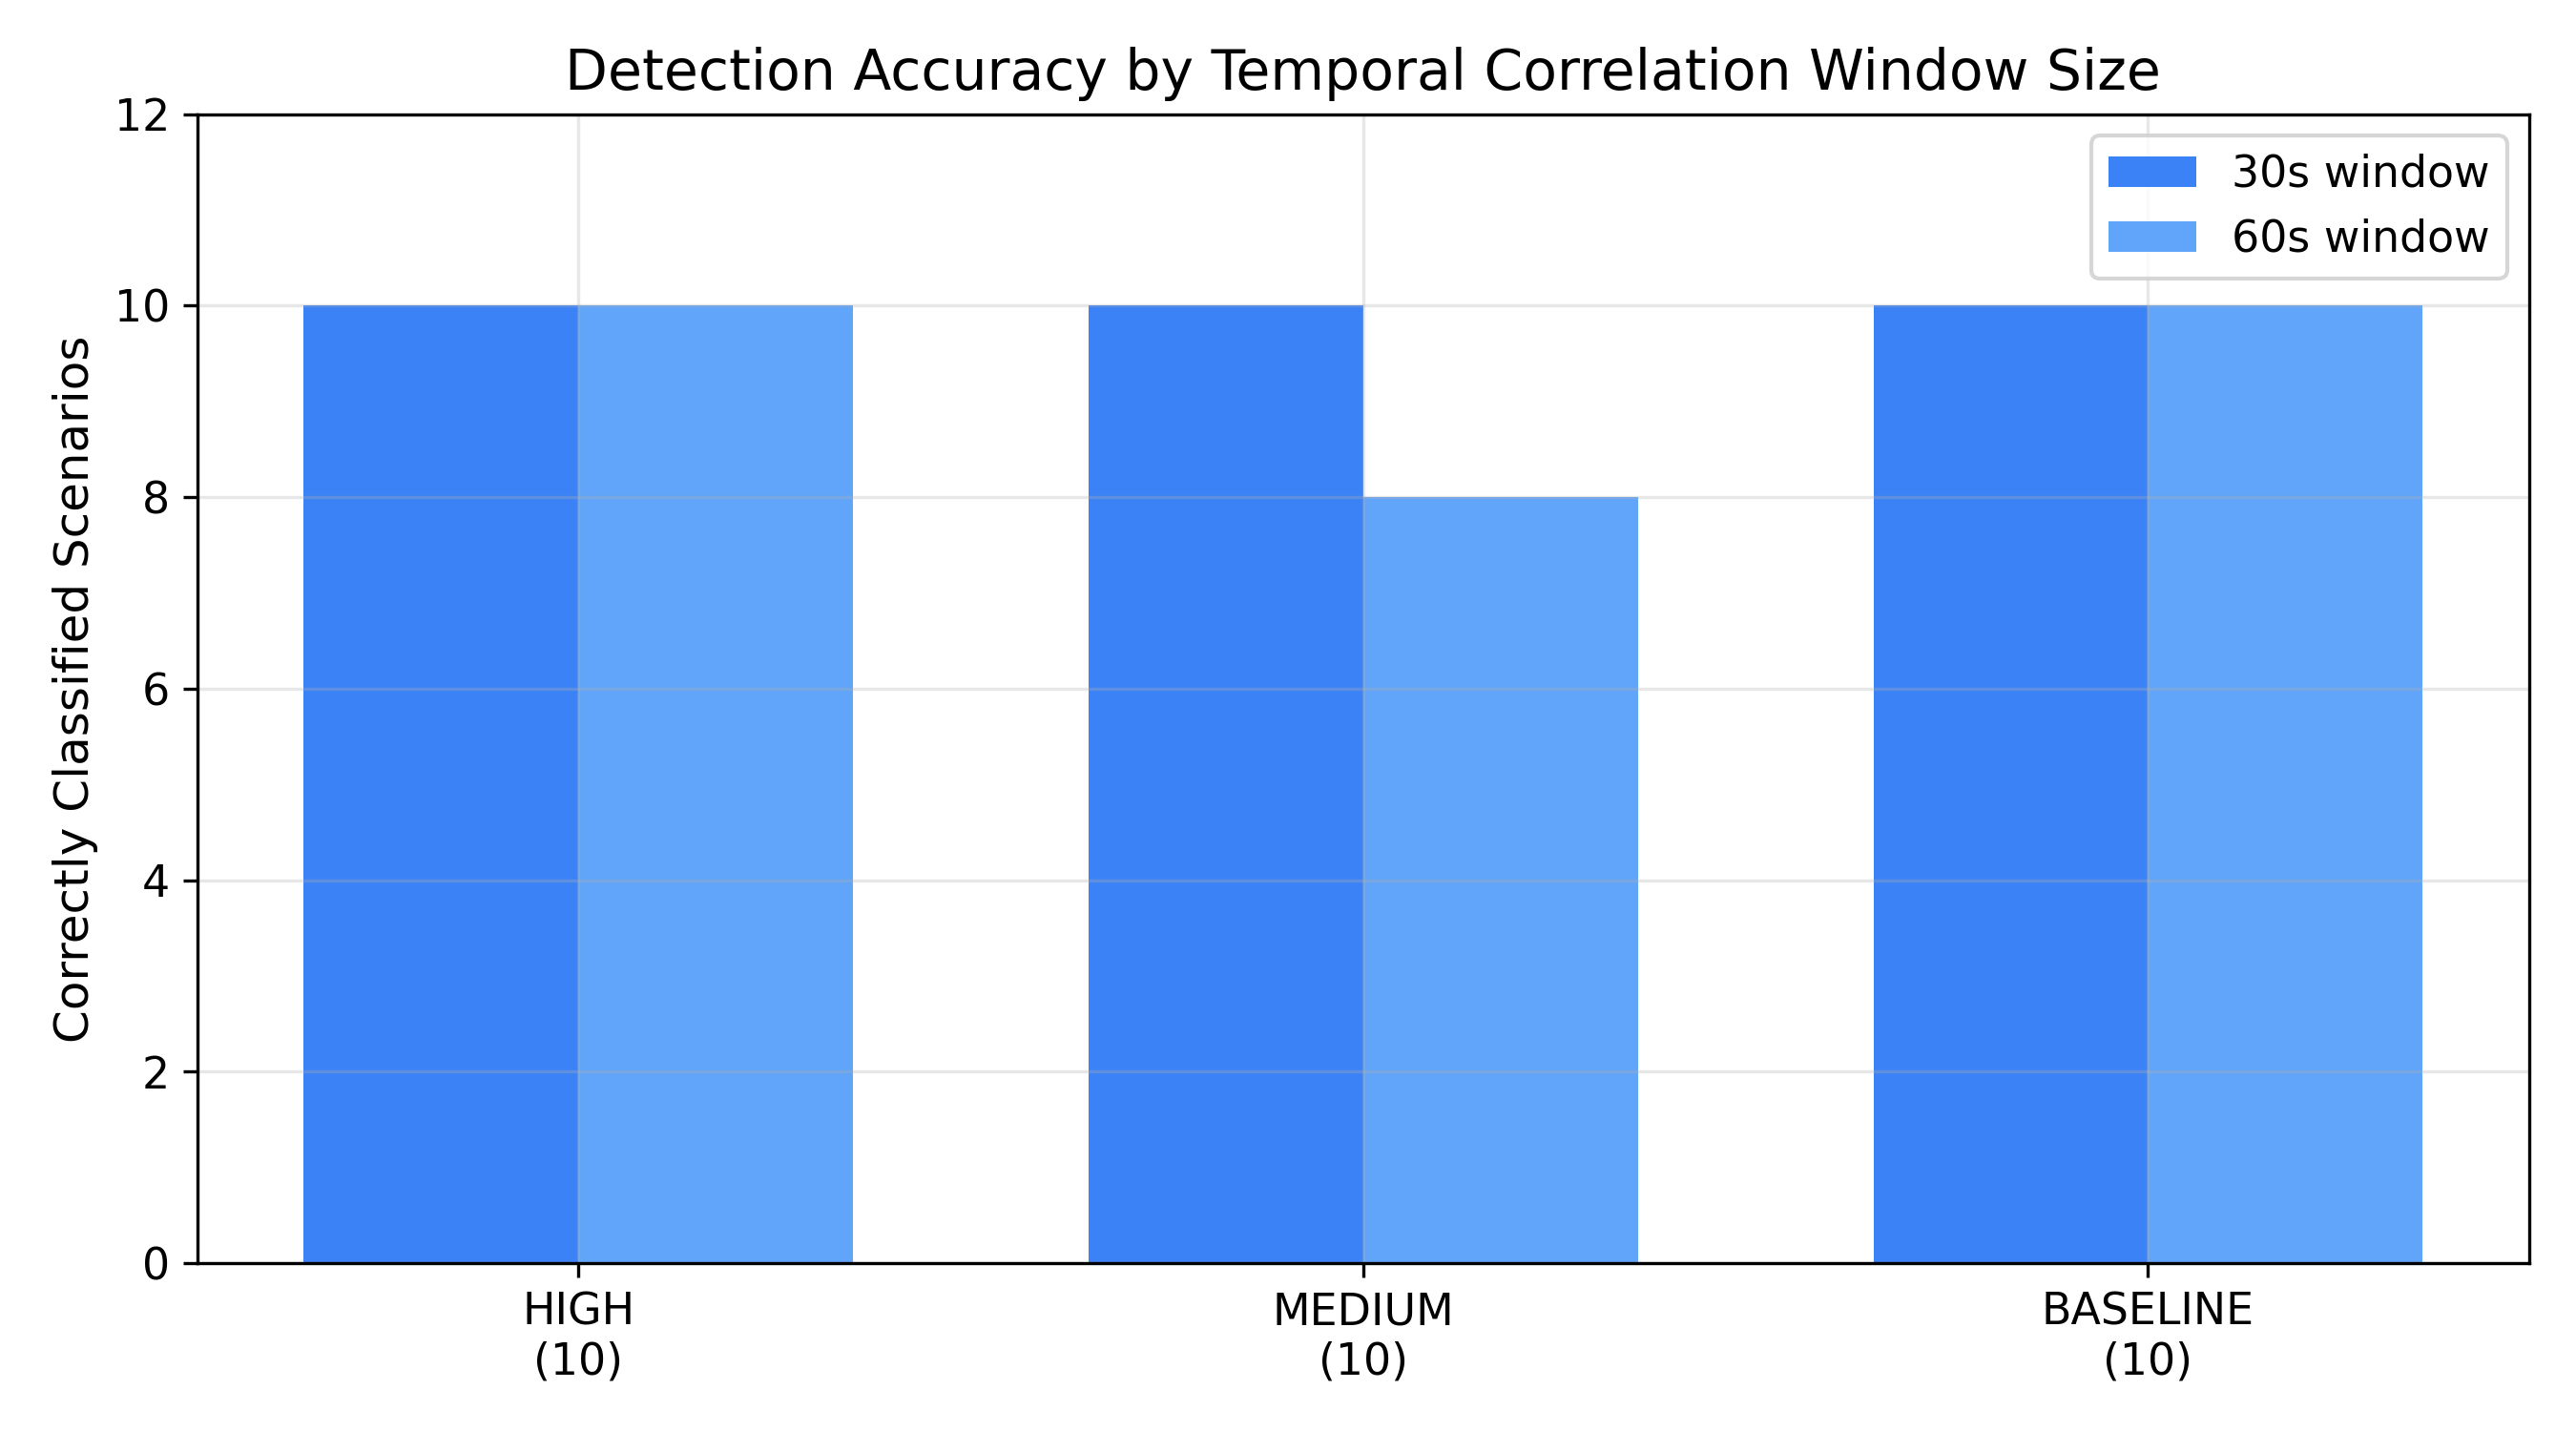
\includegraphics[width=0.9\columnwidth]{figures/fig7_window_sensitivity}}
  \caption{Detection Accuracy by Temporal Correlation Window Size. The
  30-second window achieves perfect scores at threshold 75.}
  \label{fig:window}
\end{figure}


\subsection{Analysis}

The clipboard layer was the strongest indicator (51.3 point marginal
impact). Content matching (MinHash) correctly kept scenario 16 in the
MEDIUM tier when similarity was low. The 30-second window minimized
false positives compared to 60 seconds. Scenario 19 (DPAPI-encrypted)
was correctly downgraded to MEDIUM confidence as expected.

\begin{figure}[!htbp]
  \centerline{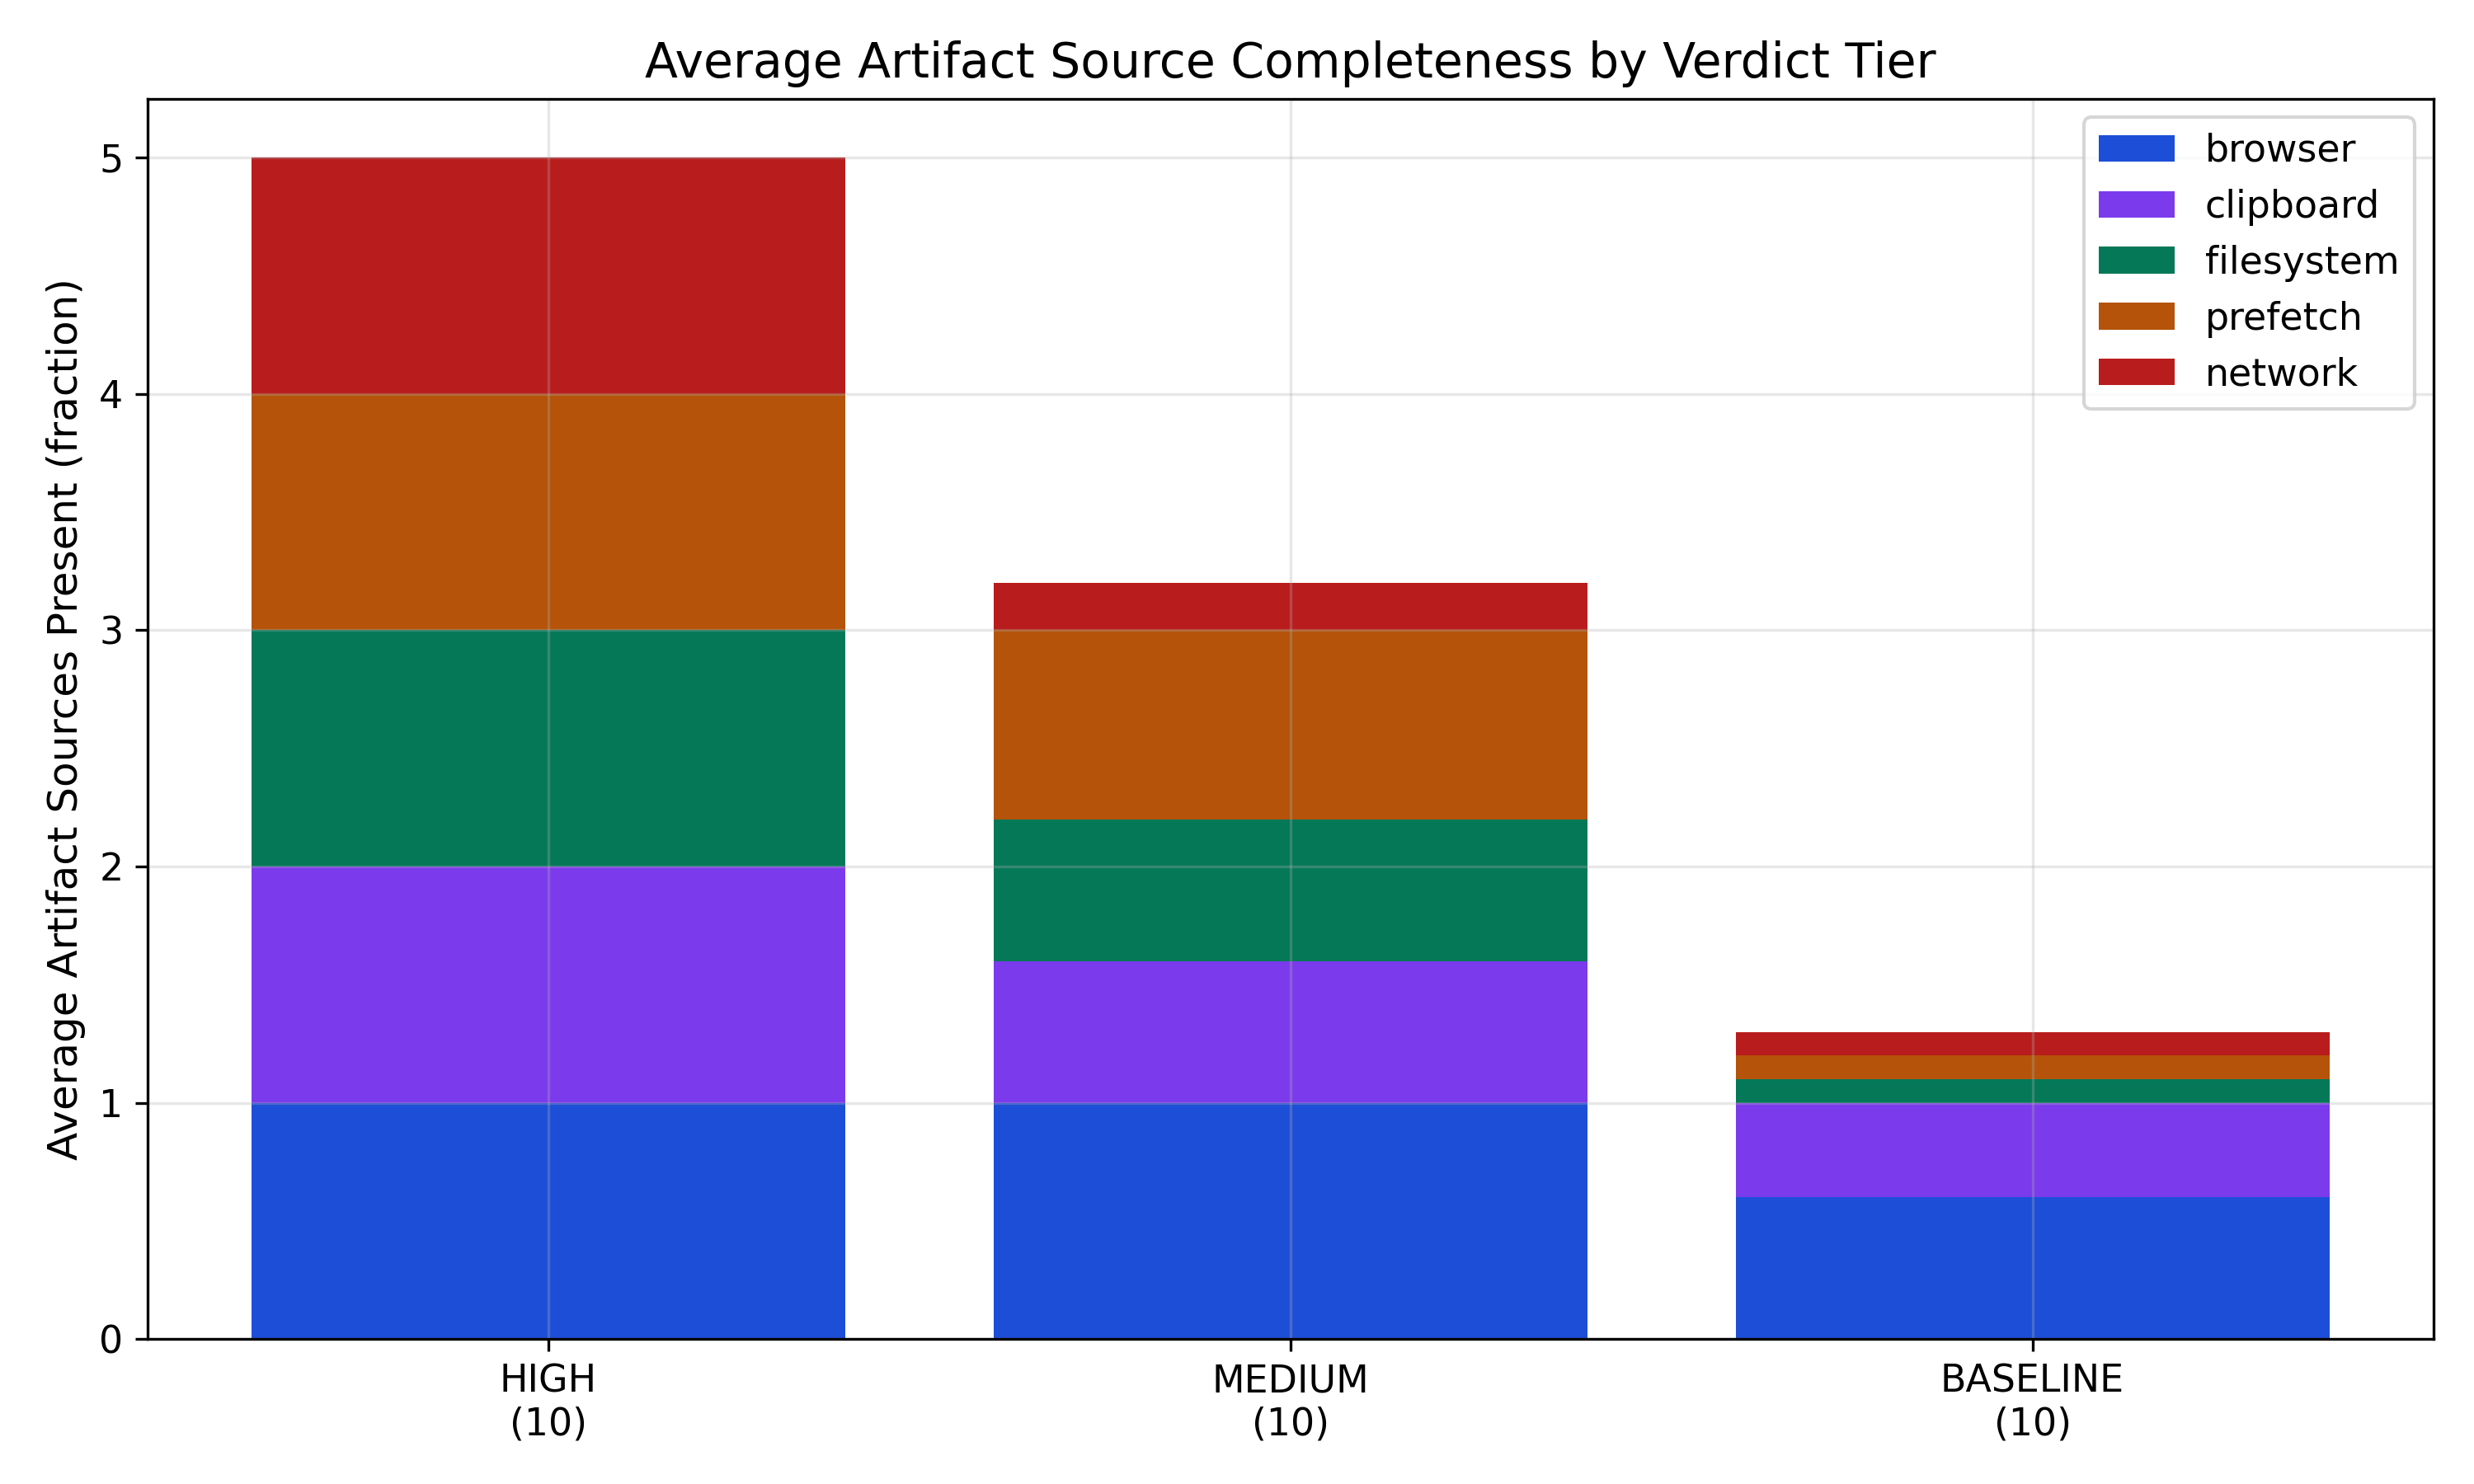
\includegraphics[width=0.9\columnwidth]{figures/fig8_source_completeness}}
  \caption{Average number of active data sources per scenario by verdict
  tier. More sources consistently means a higher tier.}
  \label{fig:source_complete}
\end{figure}


% ─────────────────────────────────────────────────────────────────────────────
%  VI. DISCUSSION
% ─────────────────────────────────────────────────────────────────────────────

\section{Discussion}
\label{sec:discussion}

No single data source is reliable enough on its own. Browser history
appeared in 26 of 30 scenarios, but alone produced an average WACS of
only 42 (weak MEDIUM). The network source produced the highest scores
when active (average 88.6), but only appeared in half the scenarios.
Combining artifacts within a short window reconstruction the copy-paste
sequence reliably.





% ─────────────────────────────────────────────────────────────────────────────
%  VII. LIMITATIONS AND FUTURE WORK
% ─────────────────────────────────────────────────────────────────────────────

\section{Limitations and Future Work}
\label{sec:limitations}

AIXFil-Detect currently works only on Windows. Future work includes
adding Volatility support for DPAPI key recovery~\cite{javed2022survey}
and extending support to macOS/Linux. As Encrypted ClientHello (ECH)
adoption grows, SNI visibility will decrease, requiring endpoint log
analysis or browser extensions~\cite{zhou2024tls}.

% ─────────────────────────────────────────────────────────────────────────────
%  VIII. CONCLUSION
% ─────────────────────────────────────────────────────────────────────────────

\section{Conclusion}
\label{sec:conclusion}

We presented AIXFil-Detect for tracing insider data theft through AI
chatbot interfaces. The tool scores correlated events using the WACS
metric. Against 30 simulated scenarios, it achieved perfect precision
and recall. The copy-paste exfiltration sequence is traceable through
synchronized Windows forensic artifacts.

% ─────────────────────────────────────────────────────────────────────────────
%  ACKNOWLEDGMENT
% ─────────────────────────────────────────────────────────────────────────────

\section*{Acknowledgment}

The authors thank Dr.~Zulfiqar Khan for his mentorship in digital
forensics and computer security.



% ─────────────────────────────────────────────────────────────────────────────
%  REFERENCES
% ─────────────────────────────────────────────────────────────────────────────

\bibliographystyle{IEEEtran}
\bibliography{aixfil_references}

\end{document}

